\documentclass[10pt]{article}  

%%%%%%%% PREÁMBULO %%%%%%%%%%%%
\title{Plantilla para prácticas de UPIITA}
\usepackage[spanish]{babel} %Indica que escribiermos en español
\usepackage[utf8]{inputenc} %Indica qué codificación se está usando ISO-8859-1(latin1)  o utf8  
\usepackage{amsmath} % Comandos extras para matemáticas (cajas para ecuaciones,
% etc)
\usepackage{amssymb} % Simbolos matematicos (por lo tanto)
\usepackage{graphicx} % Incluir imágenes en LaTeX
\usepackage{color} % Para colorear texto
\usepackage{subfigure} % subfiguras
\usepackage{float} %Podemos usar el especificador [H] en las figuras para que se
% queden donde queramos
\usepackage{capt-of} % Permite usar etiquetas fuera de elementos flotantes
% (etiquetas de figuras)
\usepackage{sidecap} % Para poner el texto de las imágenes al lado
	\sidecaptionvpos{figure}{c} % Para que el texto se alinie al centro vertical
\usepackage{caption} % Para poder quitar numeracion de figuras
\usepackage{commath} % funcionalidades extras para diferenciales, integrales,
% etc (\od, \dif, etc)
\usepackage{cancel} % para cancelar expresiones (\cancelto{0}{x})
 
\usepackage{anysize} 					% Para personalizar el ancho de  los márgenes
\marginsize{2cm}{2cm}{2cm}{2cm} % Izquierda, derecha, arriba, abajo

\usepackage{appendix}
\renewcommand{\appendixname}{Apéndices}
\renewcommand{\appendixtocname}{Apéndices}
\renewcommand{\appendixpagename}{Apéndices} 

% Para que las referencias sean hipervínculos a las figuras o ecuaciones y
% aparezcan en color
\usepackage[colorlinks=true,plainpages=true,citecolor=blue,linkcolor=blue]{hyperref}
%\usepackage{hyperref} 
% Para agregar encabezado y pie de página
\usepackage{fancyhdr} 
\pagestyle{fancy}
\fancyhf{}
\fancyhead[L]{\footnotesize UGR} %encabezado izquierda
\fancyhead[R]{\footnotesize EV}   % dereecha
\fancyfoot[R]{\footnotesize Práctica V}  % Pie derecha
\fancyfoot[C]{\thepage}  % centro
\fancyfoot[L]{\footnotesize Master en Ingeniería Informática}  %izquierda
\renewcommand{\footrulewidth}{0.4pt}

% Directorio para las imágenes
\graphicspath{{/Users/jesusgarciamanday/Desktop/Master/EV/Practicas/Practica5/p5/Imagenes/}}


\usepackage{listings} % Para usar código fuente
\definecolor{dkgreen}{rgb}{0,0.6,0} % Definimos colores para usar en el código
\definecolor{gray}{rgb}{0.5,0.5,0.5} 
% configuración para el lenguaje que queramos utilizar
\lstset{language=Matlab,
   keywords={break,case,catch,continue,else,elseif,end,for,function,
      global,if,otherwise,persistent,return,switch,try,while},
   basicstyle=\ttfamily,
   keywordstyle=\color{blue},
   commentstyle=\color{red},
   stringstyle=\color{dkgreen},
   numbers=left,
   numberstyle=\tiny\color{gray},
   stepnumber=1,
   numbersep=10pt,
   backgroundcolor=\color{white},
   tabsize=4,
   showspaces=false,
   showstringspaces=false}

\newcommand{\sen}{\operatorname{\sen}}	% Definimos el comando \sen para el seno
%en español

%%%%%%%% TERMINA PREÁMBULO %%%%%%%%%%%%

\begin{document}

%%%%%%%%%%%%%%%%%%%%%%%%%%%%%%%%%% PORTADA %%%%%%%%%%%%%%%%%%%%%%%%%%%%%%%%%%%%%%%%%%%%
																					%%%
\begin{center}																		%%%
\newcommand{\HRule}{\rule{\linewidth}{0.5mm}}									%%%\left
 																					%%%
\begin{minipage}{0.48\textwidth} \begin{flushleft}
%
\includegraphics[scale = 0.63]{Imagenes/logo_upiita}
\end{flushleft}\end{minipage}
\begin{minipage}{0.48\textwidth} \begin{flushright}
%
\includegraphics[scale = 0.35]{Imagenes/IPN}
\end{flushright}\end{minipage}

													 								%%%
\vspace*{0.25cm}								%%%
																					%%%	
\textsc{\huge Universidad de Granada}\\[1.5cm]	

\textsc{\LARGE Master en Ingeniería Informática}\\[1.5cm]													%%%

\textsc{\LARGE Entornos Virtuales}\\[1.5cm]													%%%

\begin{minipage}{0.9\textwidth} 
\begin{center}																					%%%
\textsc{\LARGE Practica V}
\end{center}
\end{minipage}\\[0.5cm]
%%%
    																				%%%
 			\vspace*{1cm}																		%%%
																					%%%
\HRule \\[0.4cm]																	%%%
{ \huge \bfseries Simulación}\\[0.4cm]	%%%
 																					%%%
\HRule \\[1.5cm]																	%%%
 																				%%%
																					%%%
\begin{minipage}{0.46\textwidth}													%%%
\begin{flushleft} \large															%%%
\emph{Autor:}\\	
 Manuel Jesús García Manday
%%%
			%\vspace*{2cm}	
            													%%%
										 						%%%
\end{flushleft}																		%%%
\end{minipage}		
																%%%
\begin{minipage}{0.52\textwidth}		
\vspace{-0.6cm}											%%%
\begin{flushright} \large															%%%													%%%
\end{flushright}																	%%%
\end{minipage}	
\vspace*{1cm}
%\begin{flushleft}
 	
%\end{flushleft}
%%%
 		\flushleft{\textbf{\Large Master en Ingeniería Informática}	}\\																		%%%
\vspace{2cm} 																				
\begin{center}																					

%{\large \today}																	%%%
 			\end{center}												  						
\end{center}							 											
																					
\newpage																		
%%%%%%%%%%%%%%%%%%%% TERMINA PORTADA %%%%%%%%%%%%%%%%%%%%%%%%%%%%%%%%

\tableofcontents 

\newpage

\section{Objetivo.}
El objetivo de esta práctica es aprender a utilizar el motor de física de Blender.


\section{Desarrollo de la práctica.}
Se ha planteado el siguiente escenario donde se van a realizar las simulaciones utilizando para ello el motor físico \textbf{Bullet}. En dicha simulación el objeto ``Coche'' se desplazará hacia el objeto ``Mundo'' colisionando contra el y produciendo que se desarme por motivo del impacto. \\

\begin{figure}[H]
	\begin{center}
	 		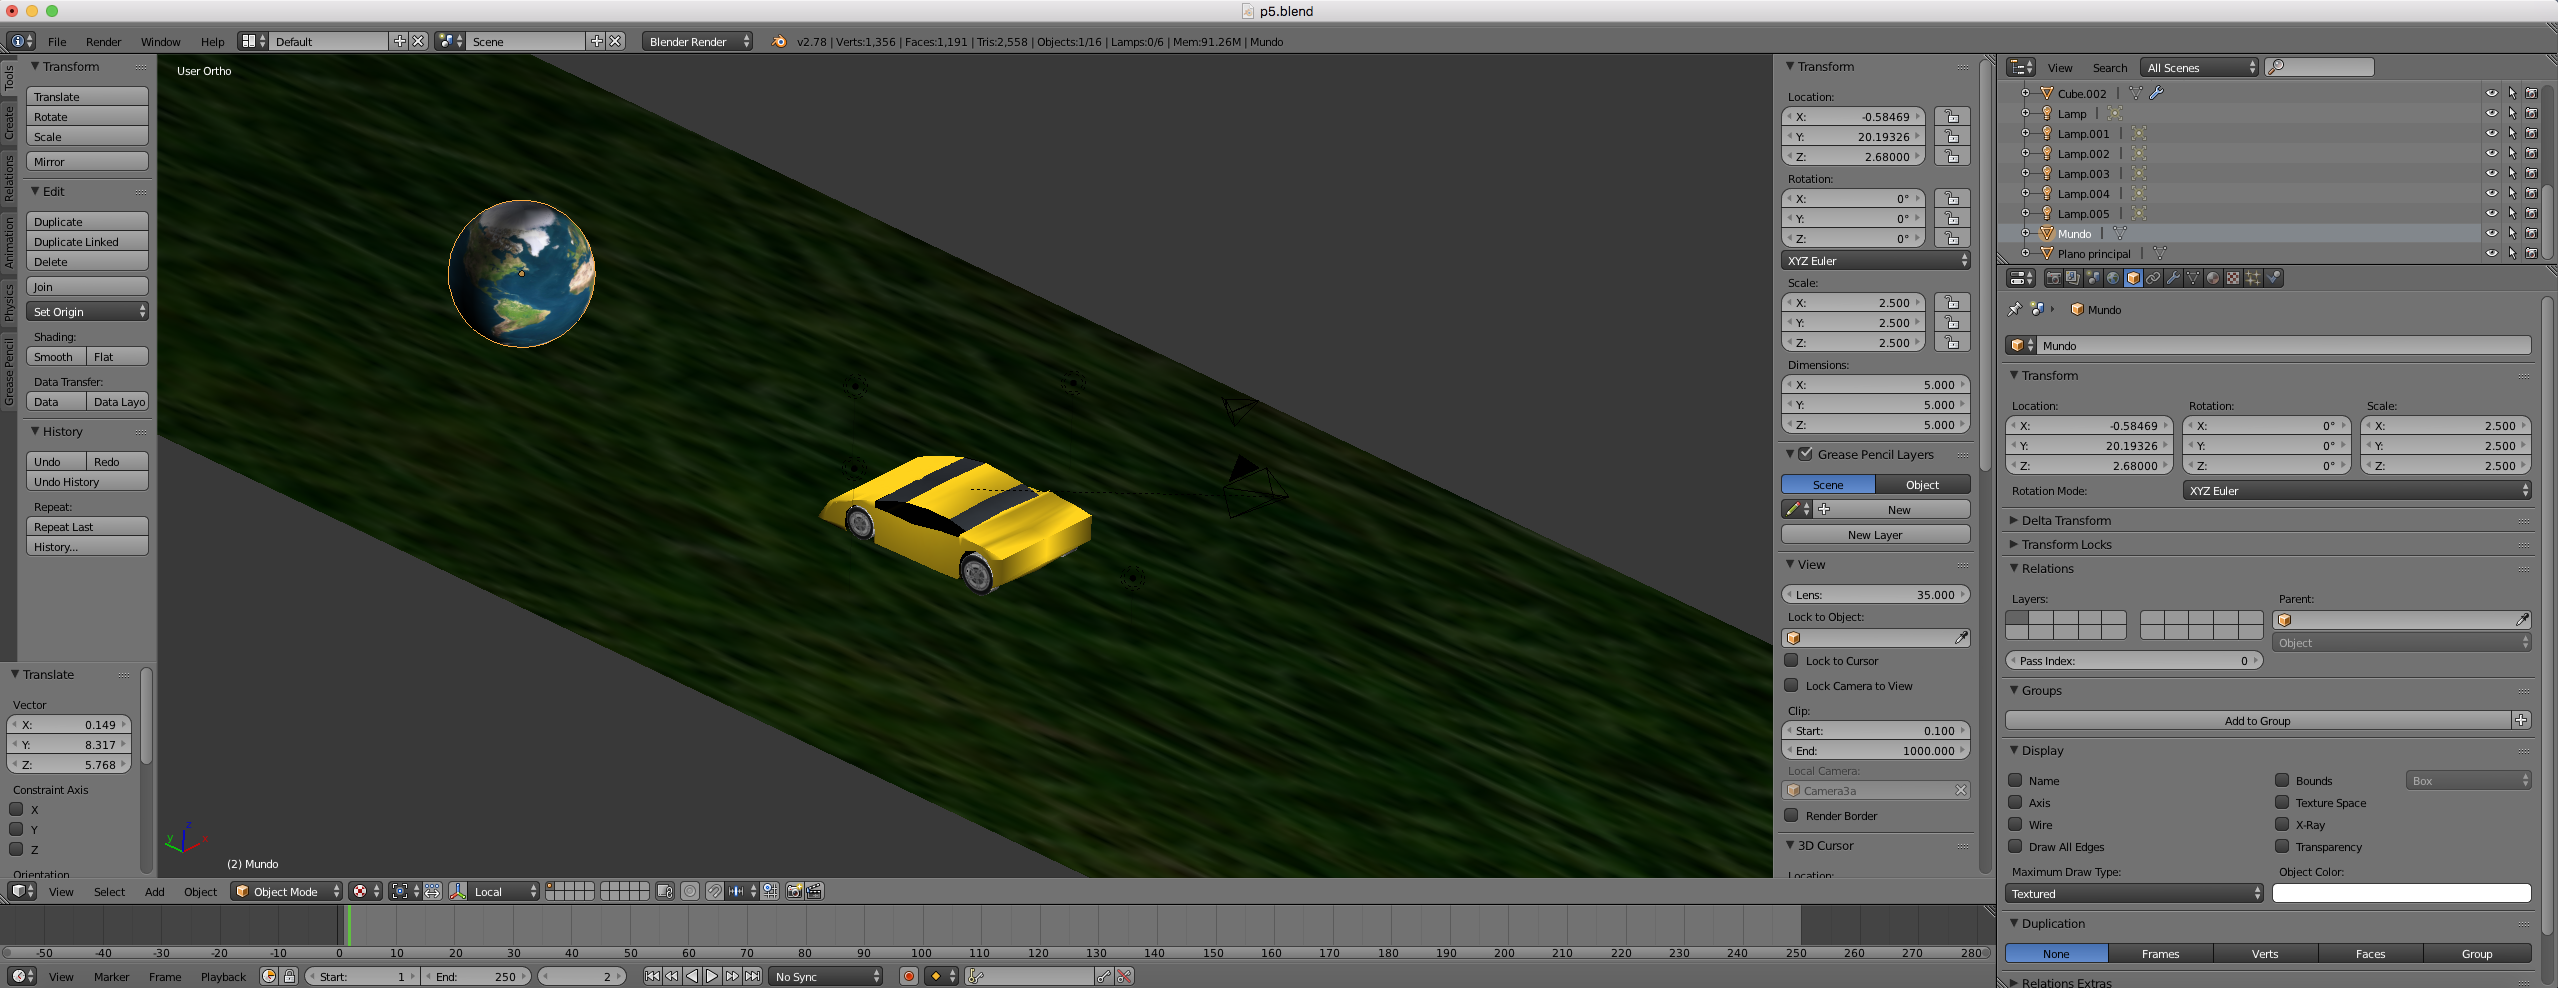
\includegraphics[width = 1.00\textwidth]{Imagenes/p5-img1}
 		\captionof{figure}{\label{fig:IPN}Escenario (I).} 
	\end{center} 
\end{figure}

\begin{figure}[H]
	\begin{center}
	 		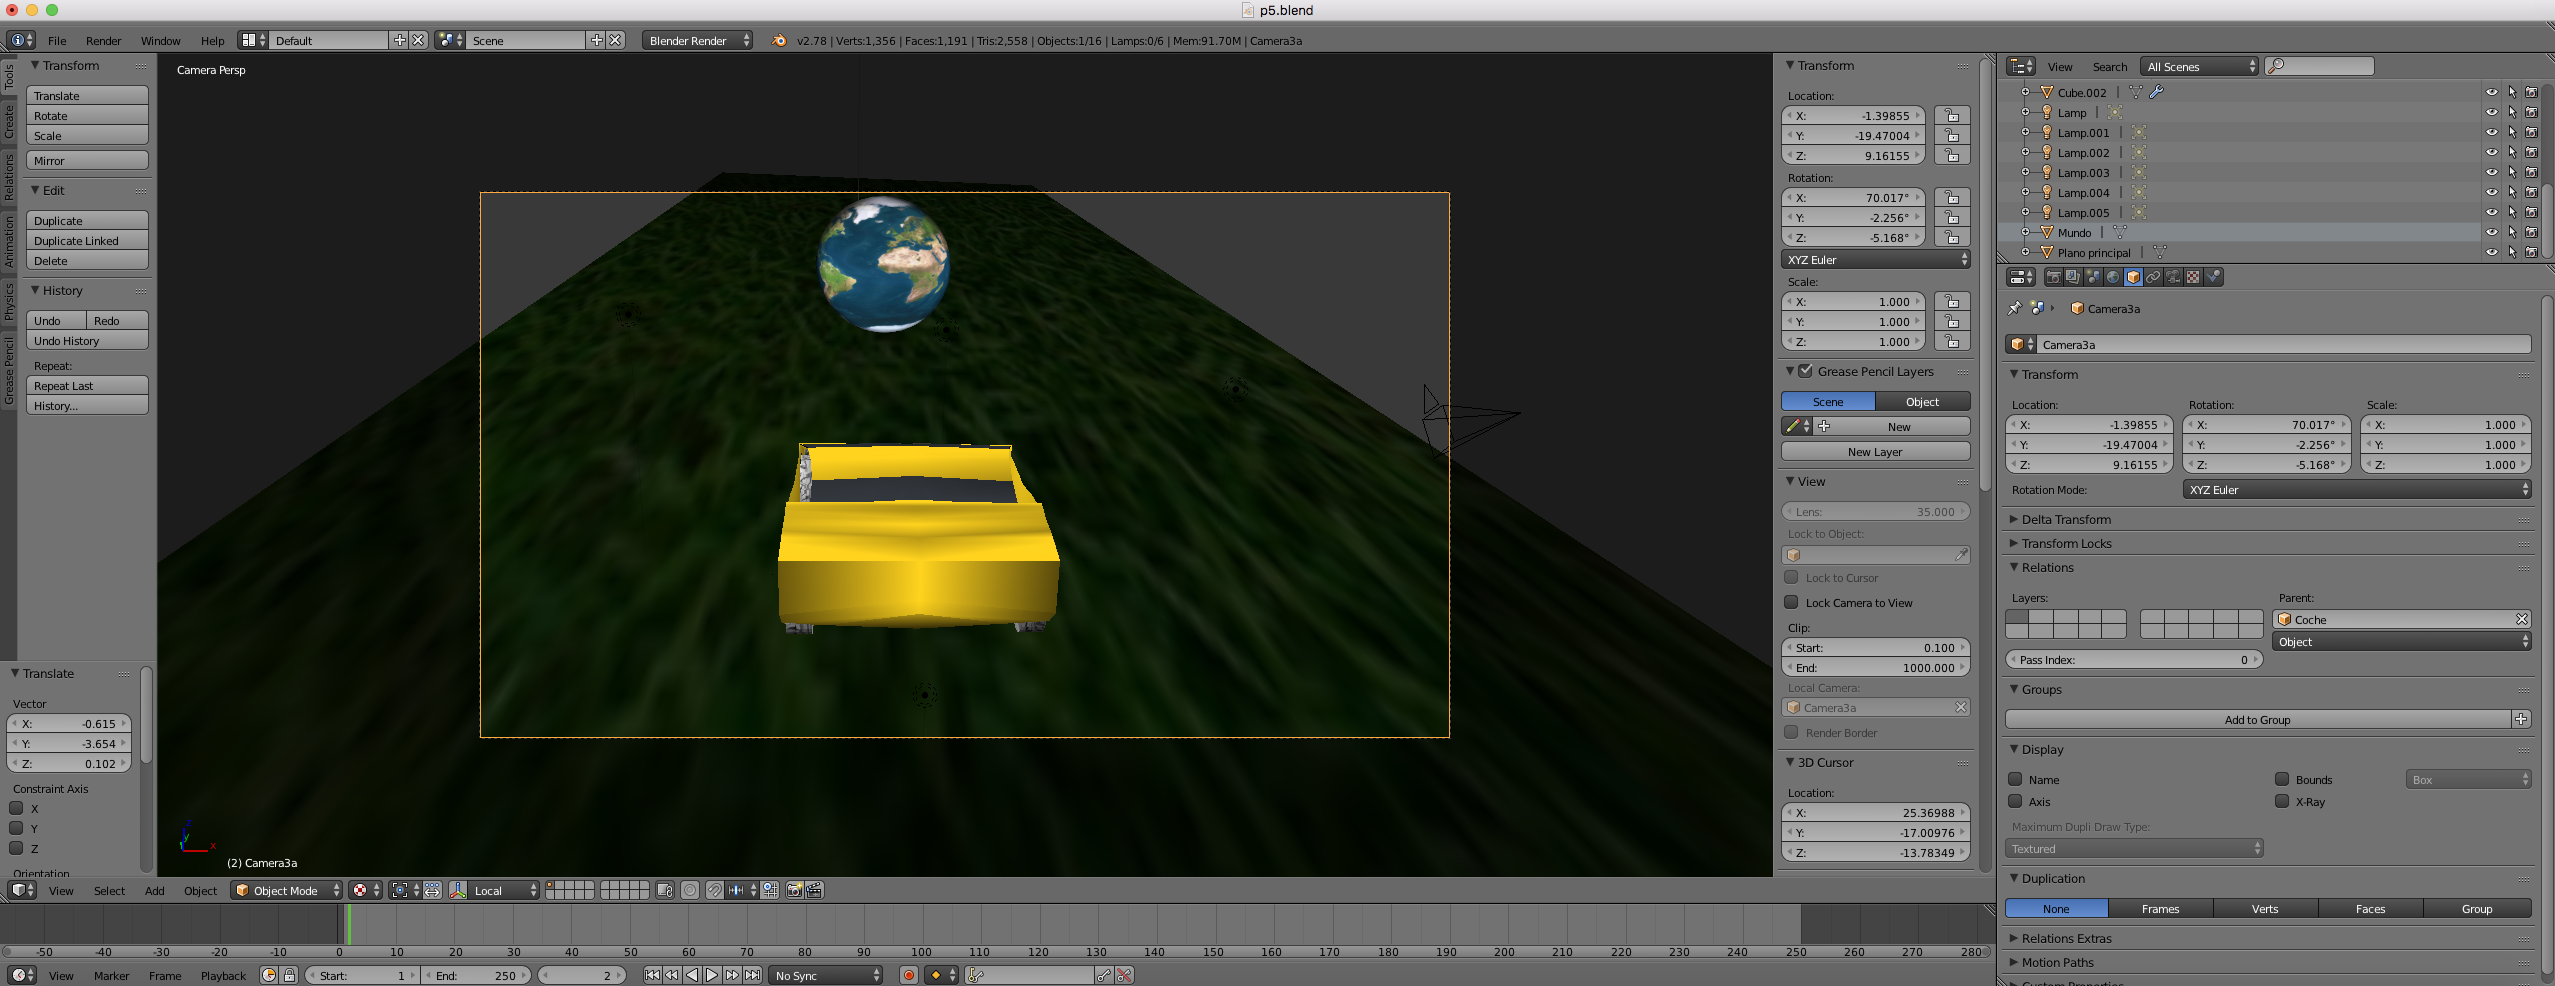
\includegraphics[width = 1.00\textwidth]{Imagenes/p5-img2}
 		\captionof{figure}{\label{fig:IPN}Escenario (II).} 
	\end{center} 
\end{figure}

Lo primero que necesitamos hacer es añadir la opción \textbf{cell fracture} para poder hacer que la esfera que representa el ``Mundo'' de desarme cuando el objeto ``Coche'' colisione contra ella. Para ello vamos a \textbf{File -- User preferences -- Add-ons} lo buscamos y los guardamos en nuestra configuración como se muestra en la siguiente imagen. \\

\begin{figure}[H]
	\begin{center}
	 		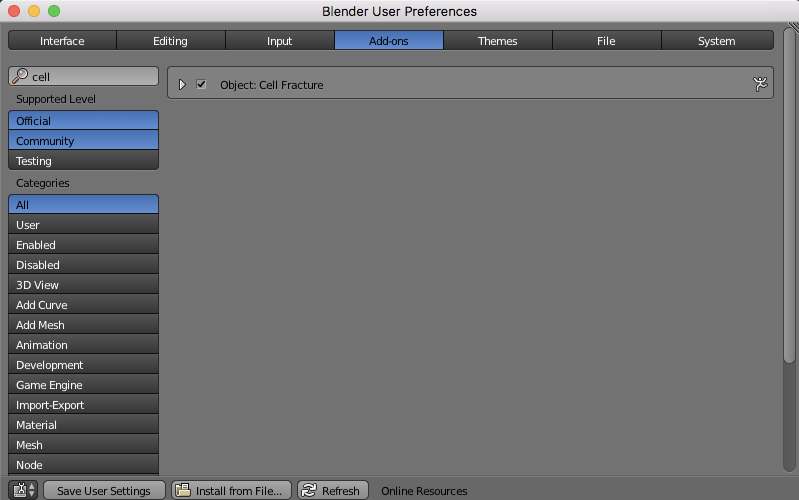
\includegraphics[width = 1.00\textwidth]{Imagenes/p5-img3}
 		\captionof{figure}{\label{fig:IPN}Añadiendo ``cell fracture'').} 
	\end{center} 
\end{figure}

Con los objetos colocados en el escenario como se ha visto en las \textbf{figuras 1} y \textbf{2}, pasamos a emparentarlos haciendo al objeto ``Coche'' hijo del objeto ``Esfera''. \\

\begin{figure}[H]
	\begin{center}
	 		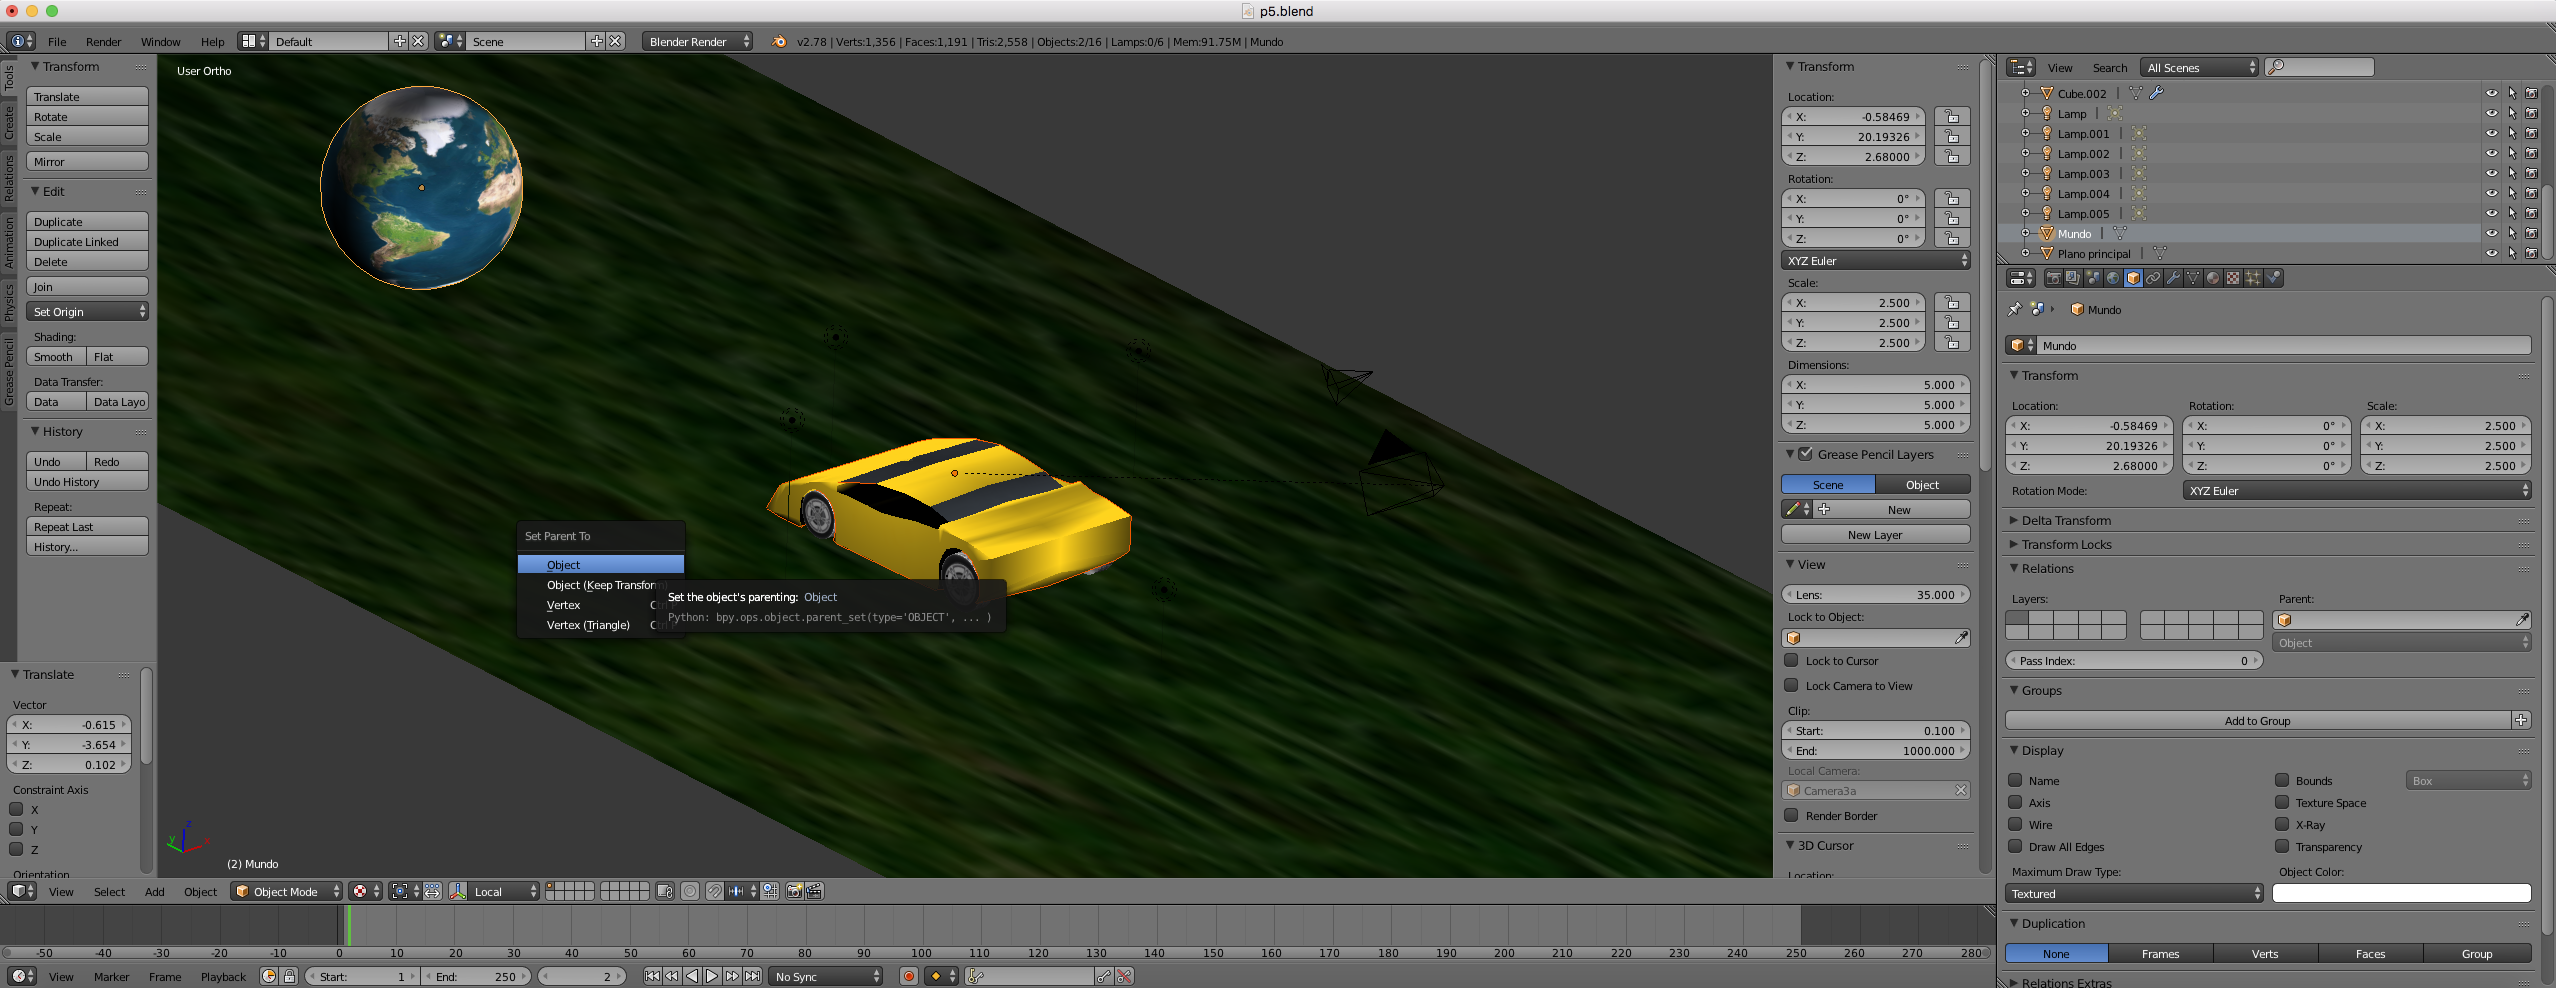
\includegraphics[width = 1.00\textwidth]{Imagenes/p5-img4}
 		\captionof{figure}{\label{fig:IPN}Emparentando los objetos).} 
	\end{center} 
\end{figure}

Ahora pasamos a modo alambre y unimos ambos objetos para indicar cómo y donde será la colisión del objeto ``Coche'' con el objeto ``Mundo''. Es neceario también añadirle al objeto ``Mundo'' un modificador de tipo \textbf{Solidify} para que no se desarme con relleno, para lo que hay que aunmentar el valor del grosor (\textbf{Thickness}) a \textbf{0.0280} como se muetra en la siguiente figura.\\

\begin{figure}[H]
	\begin{center}
	 		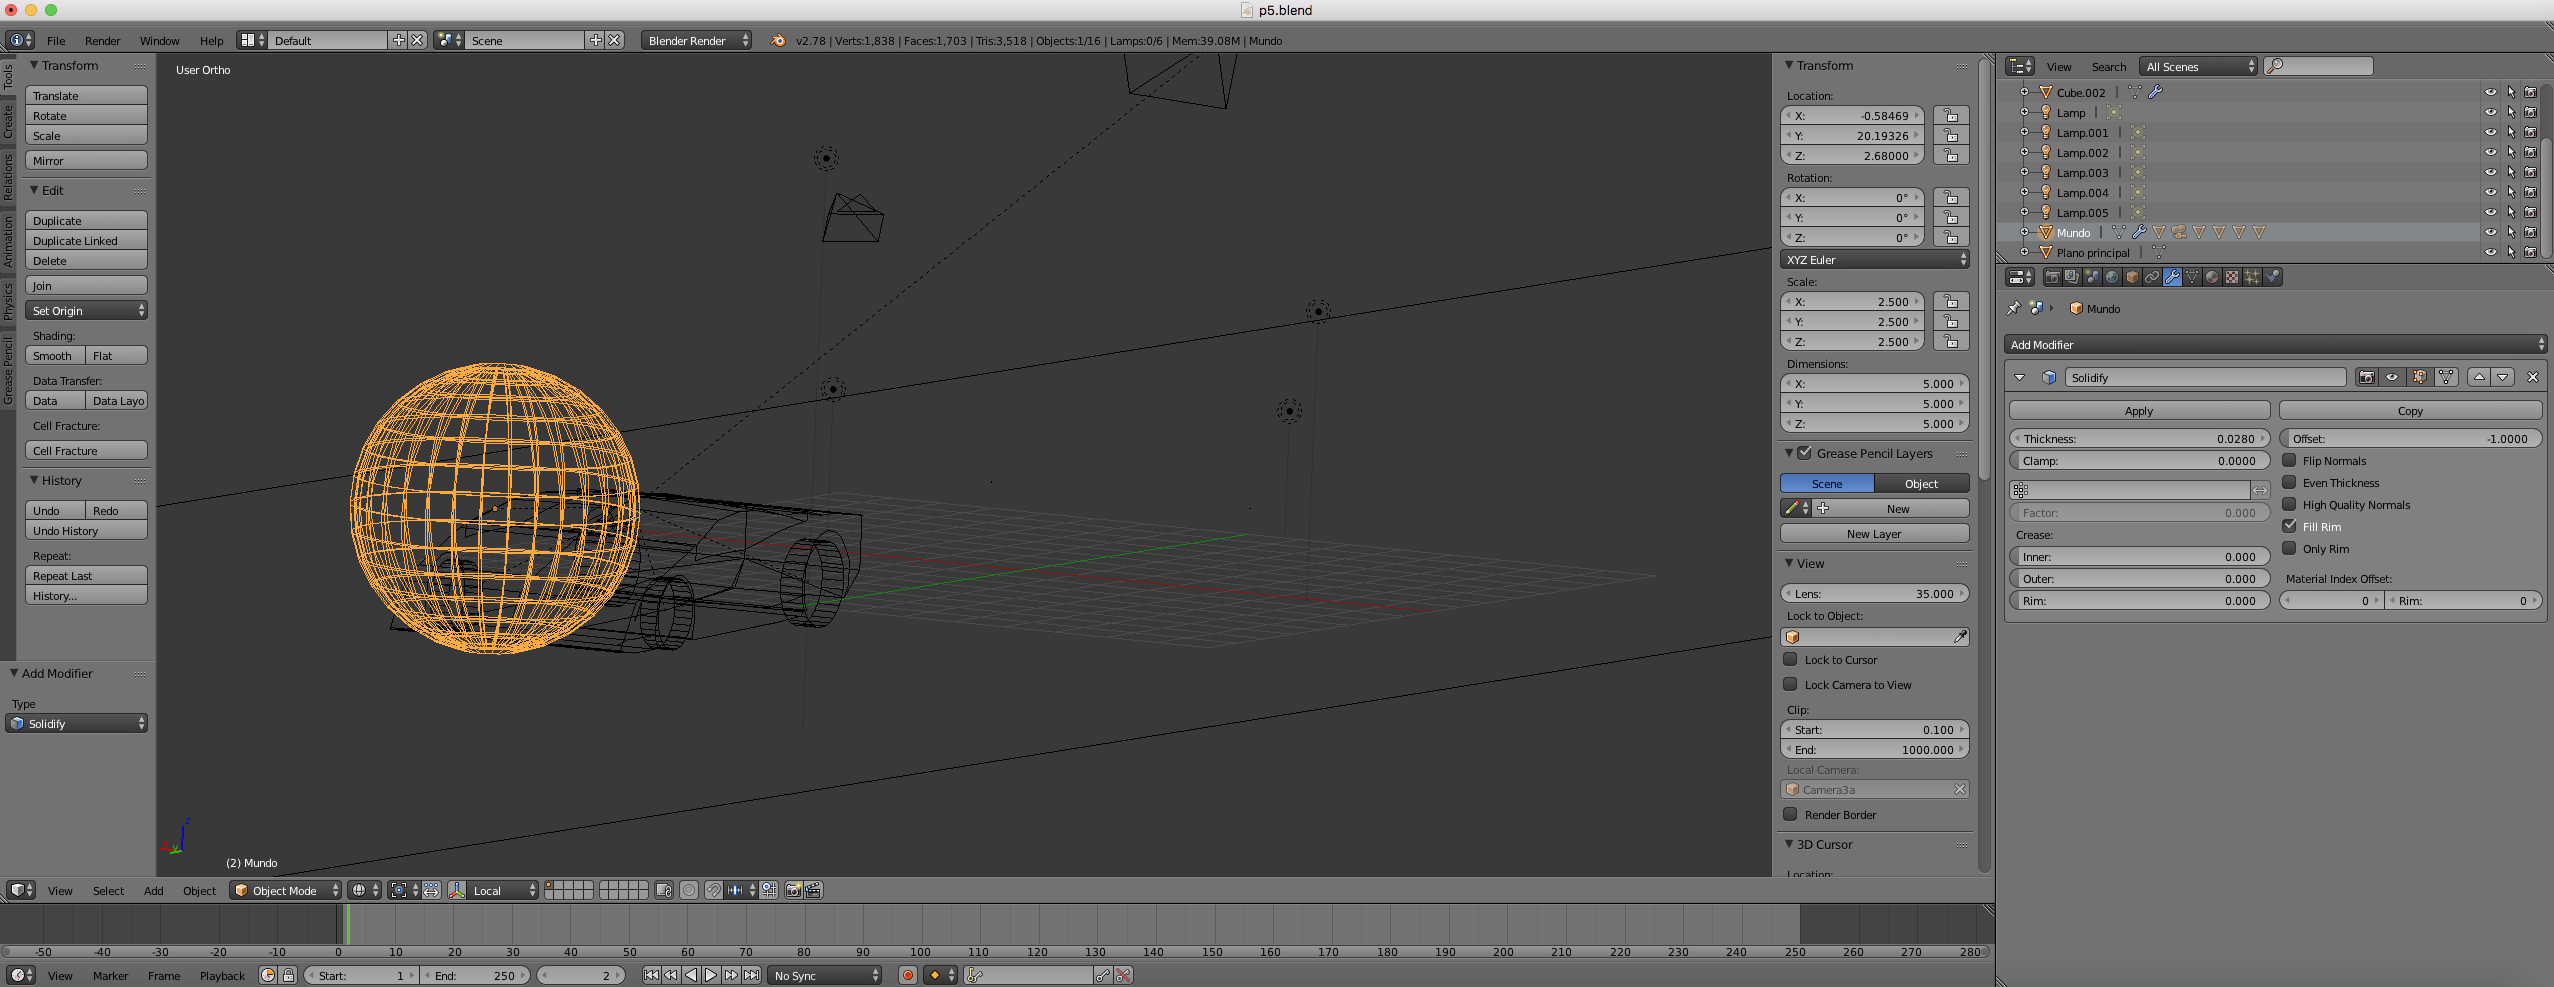
\includegraphics[width = 1.00\textwidth]{Imagenes/p5-img5}
 		\captionof{figure}{\label{fig:IPN}Aplicando modificador \textbf{Solidify}.} 
	\end{center} 
\end{figure}

Acomodamos la cámara para que se vea bien los dos objetos. \\

\begin{figure}[H]
	\begin{center}
	 		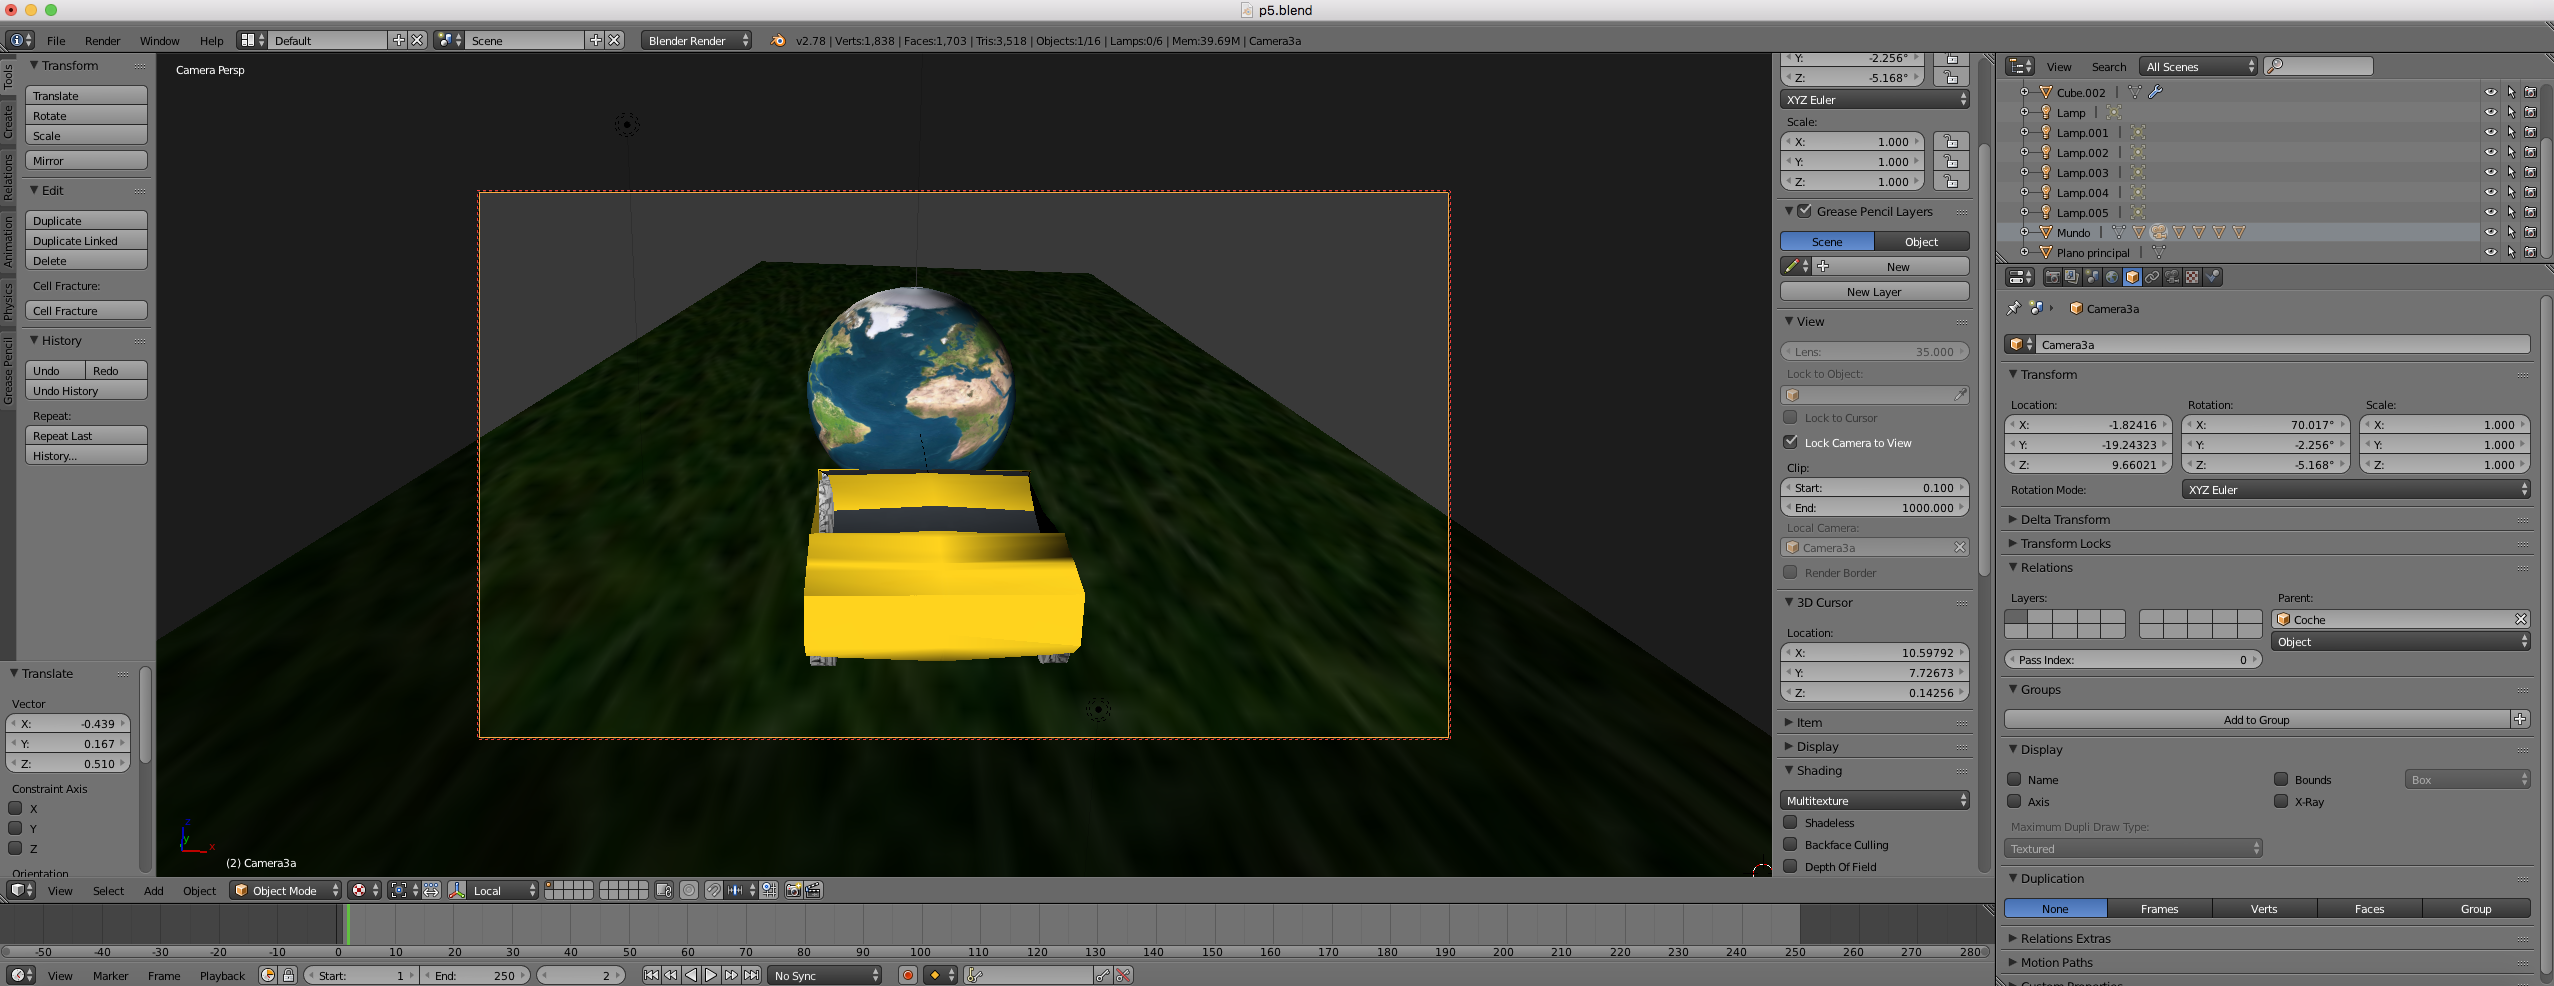
\includegraphics[width = 1.00\textwidth]{Imagenes/p5-img6}
 		\captionof{figure}{\label{fig:IPN}Acomodando la cámara.} 
	\end{center} 
\end{figure}

En la siguiente imagen se muestra el proceso de la opción \textbf{cell fracture} con la que hacemos que el objeto ``Mundo'' se desarme. Configuramos algunos parámetros de dicha fractura como el número de particiones en las que quedará el objeto. \\

\begin{figure}[H]
	\begin{center}
	 		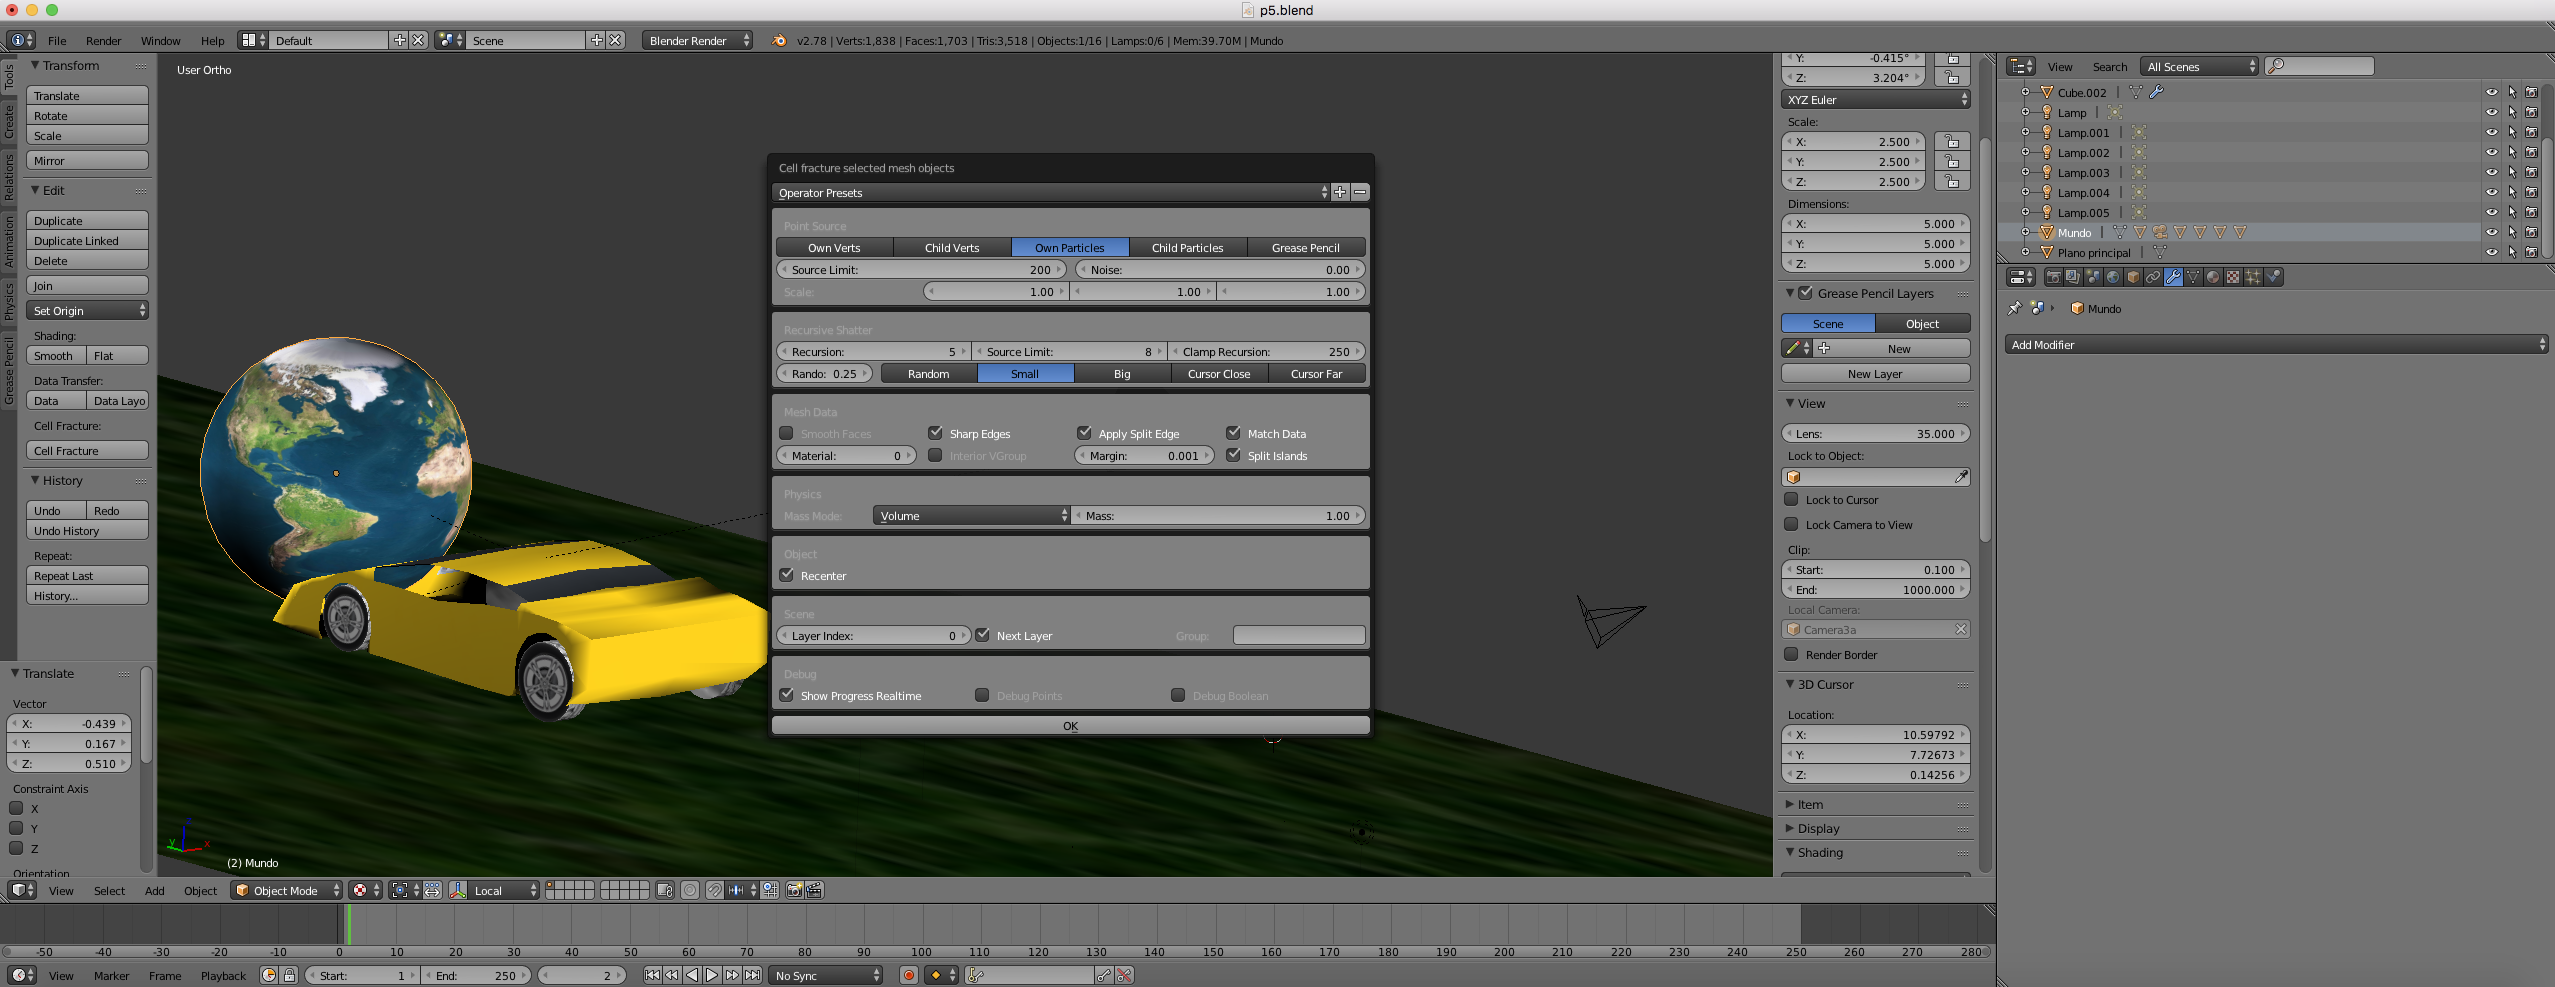
\includegraphics[width = 1.00\textwidth]{Imagenes/p5-img7}
 		\captionof{figure}{\label{fig:IPN}Configurando cell fracture.} 
	\end{center} 
\end{figure}

Al terminar este proceso podemos comprobar como ha aparecido un nuevo objeto en una segunda capa. Accedemos a dicho objeto y lo ponemos en modo alambre para que podamos ver que esta fracturado en varias particiones. También se puede comprobar en modo sólido como muestran las siguientes imágenes. \\

\begin{figure}[H]
	\begin{center}
	 		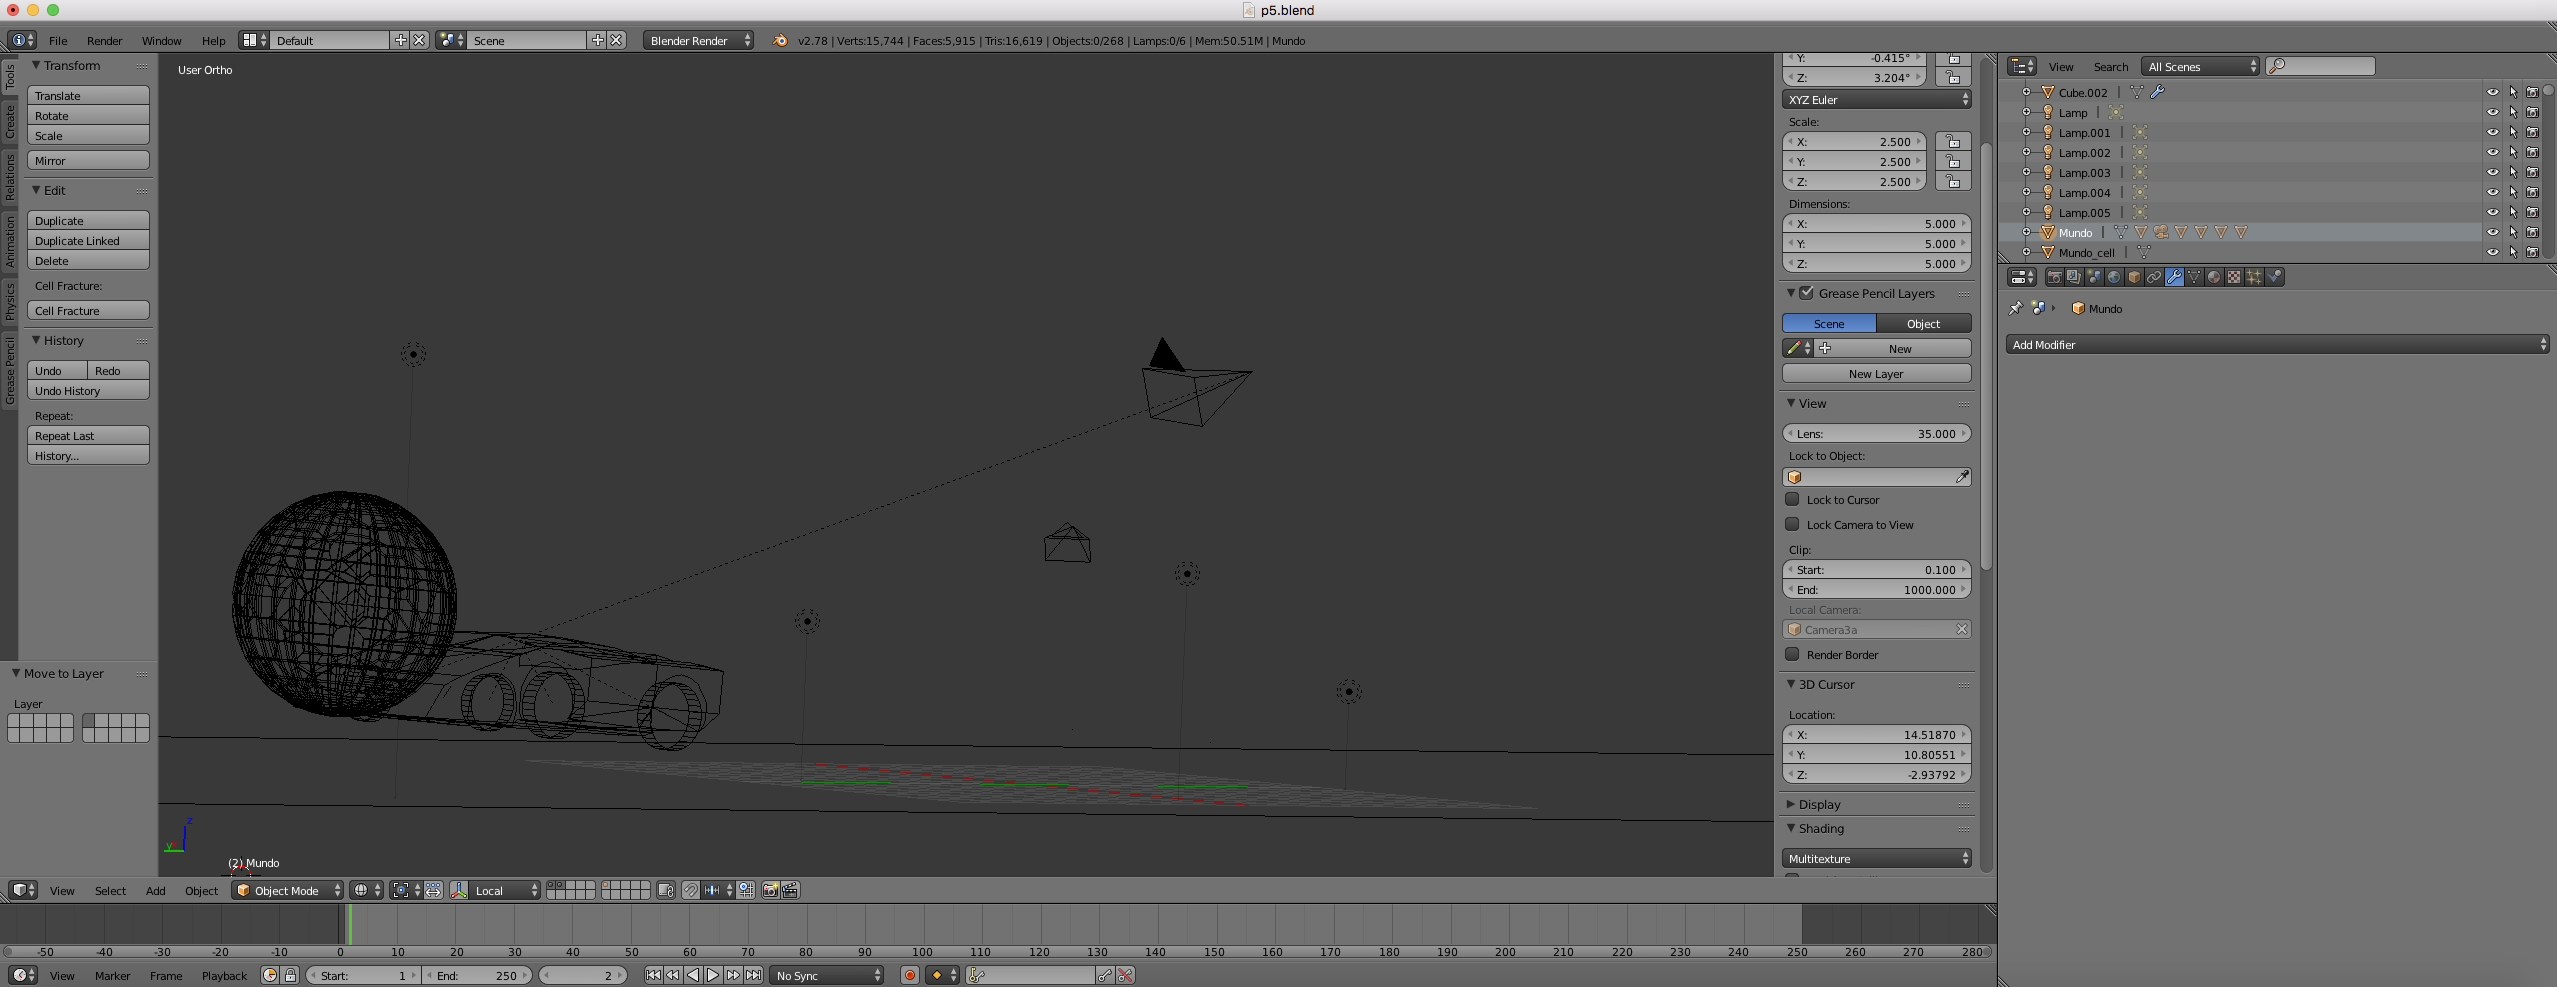
\includegraphics[width = 1.00\textwidth]{Imagenes/p5-img8}
 		\captionof{figure}{\label{fig:IPN}Visualizando objeto fracturado (I).} 
	\end{center} 
\end{figure}

\begin{figure}[H]
	\begin{center}
	 		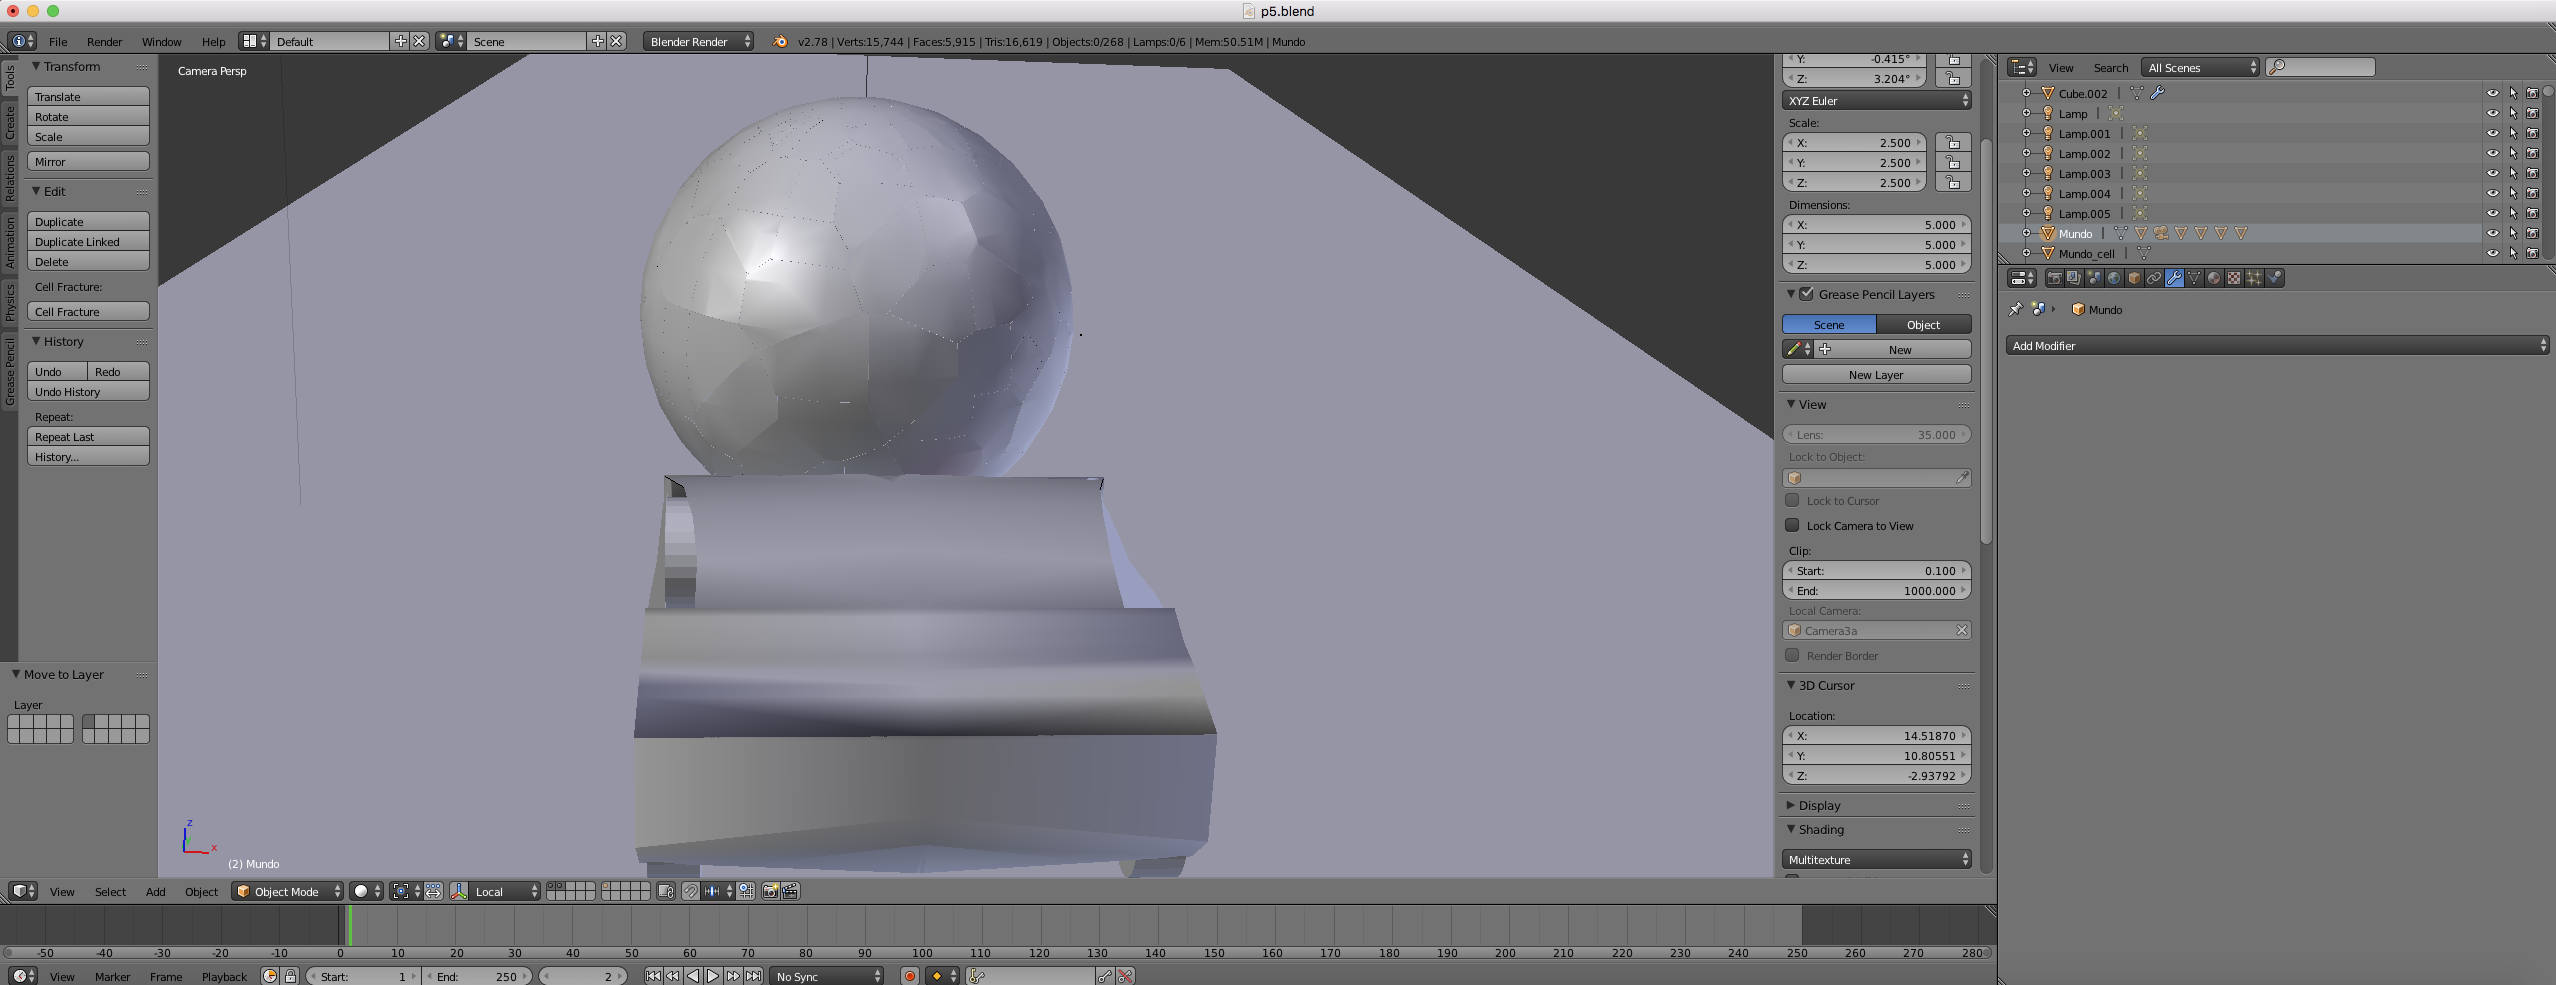
\includegraphics[width = 1.00\textwidth]{Imagenes/p5-img9}
 		\captionof{figure}{\label{fig:IPN}Visualizando objeto fracturado (II).}
	\end{center} 
\end{figure}

Nos cambiamos a la capa donde se encuentra solamente el objeto esfera que representa al ``Mundo'' para establecer la física como activa. Para ello seleccionamos todas las particiones pulsando la tecla \textbf{A}, y en el pane de \textbf{Physics} le indicamos que la añada (\textbf{Add Active}). \\

\begin{figure}[H]
	\begin{center}
	 		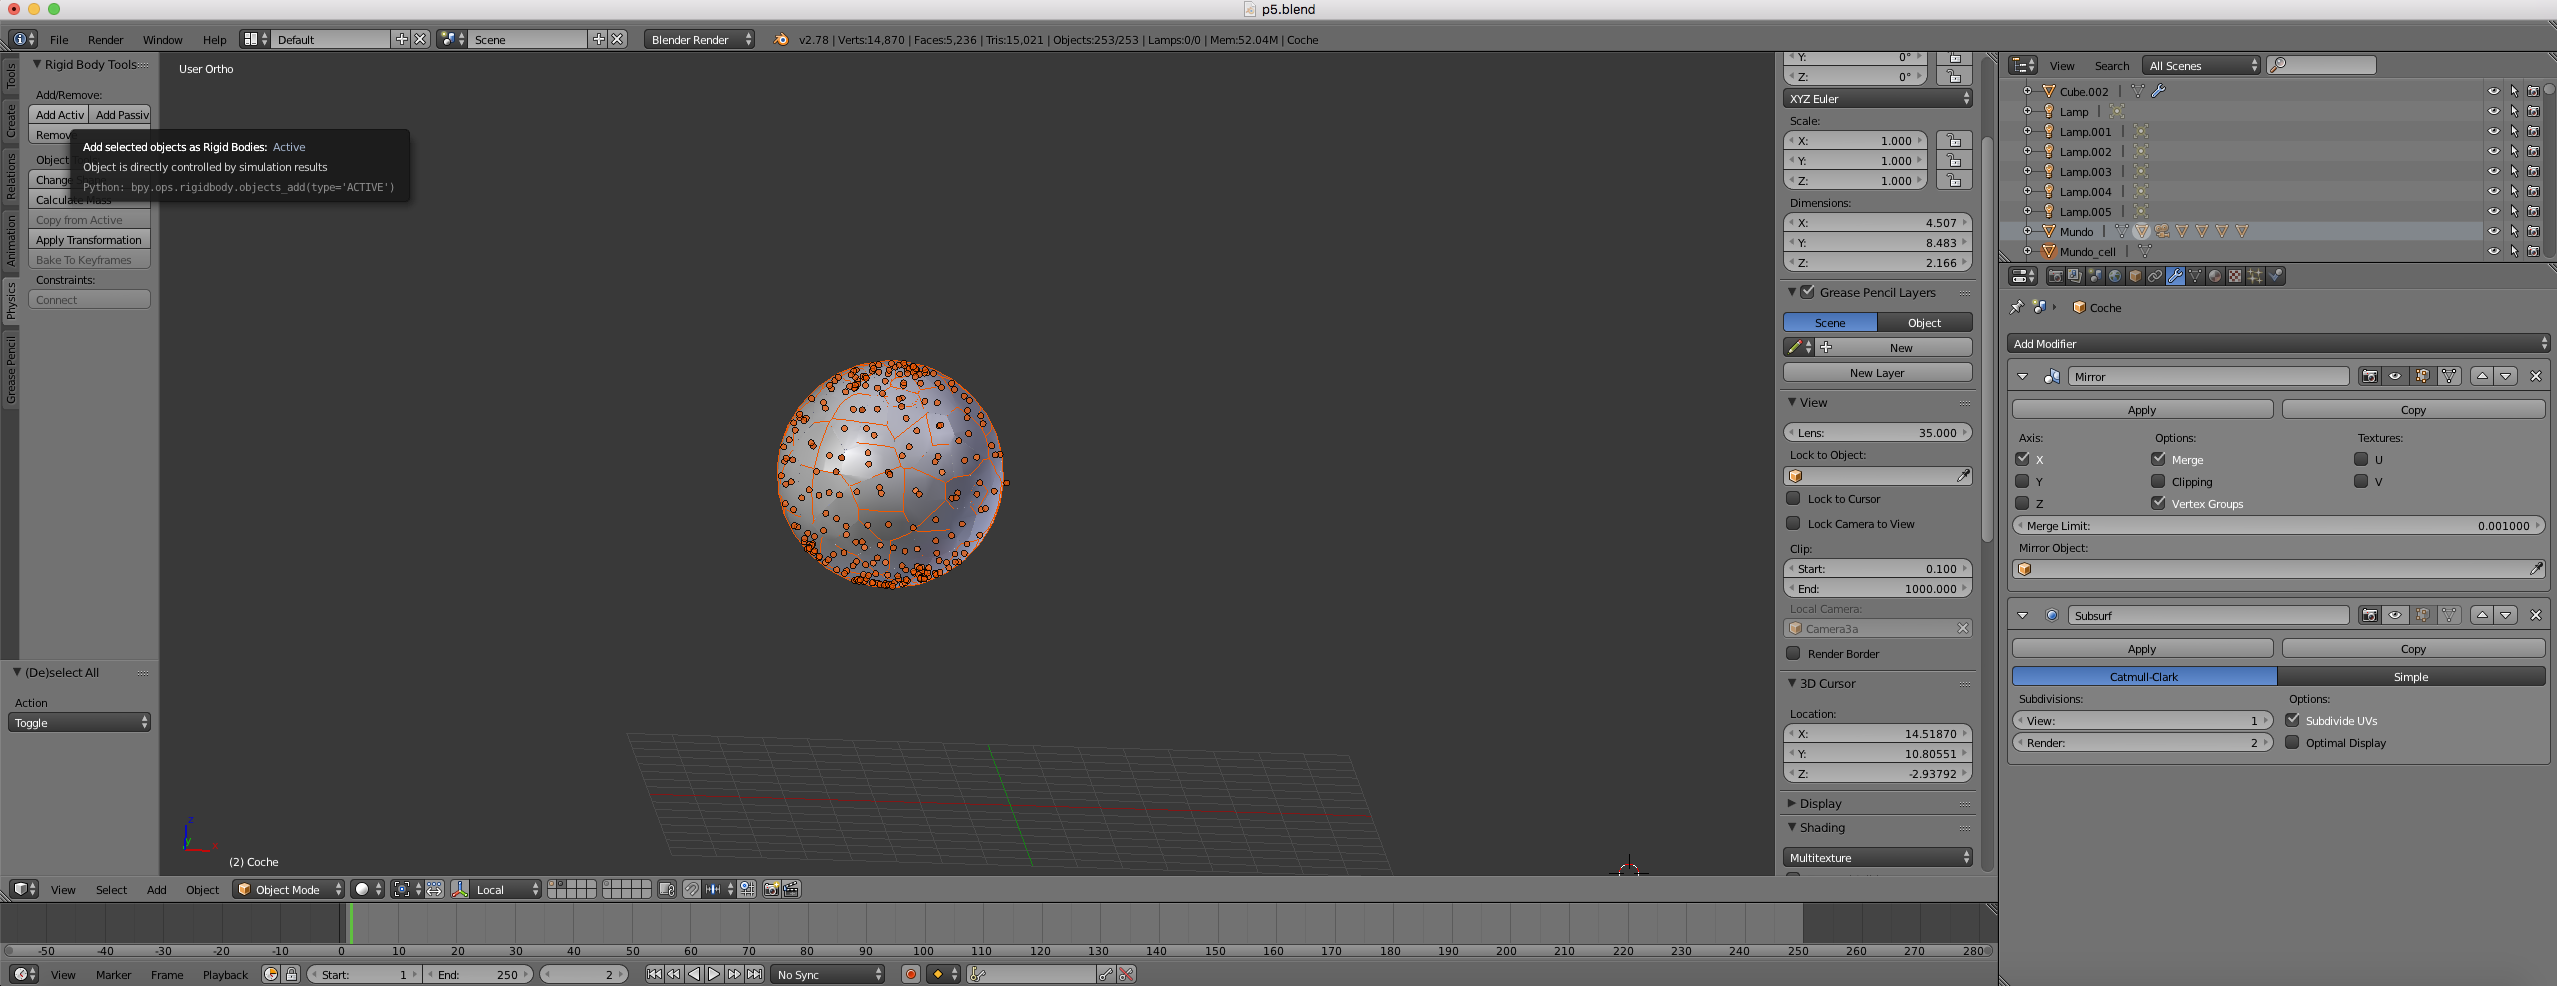
\includegraphics[width = 1.00\textwidth]{Imagenes/p5-img10}
 		\captionof{figure}{\label{fig:IPN}Estableciendo física activa al objeto ``Mundo''.}
	\end{center} 
\end{figure}

Para que la esfera no se desplace en el eje Z hasta el infinito tenemos que dar al modelo suelo la propiedad de cuerpo rígido, para ello lo seleccionamos y en el mismo panel que antes (\textbf{Physics}) le indicamos que le establezca un física pasiva (\textbf{Add Pasive}).\\

\begin{figure}[H]
	\begin{center}
	 		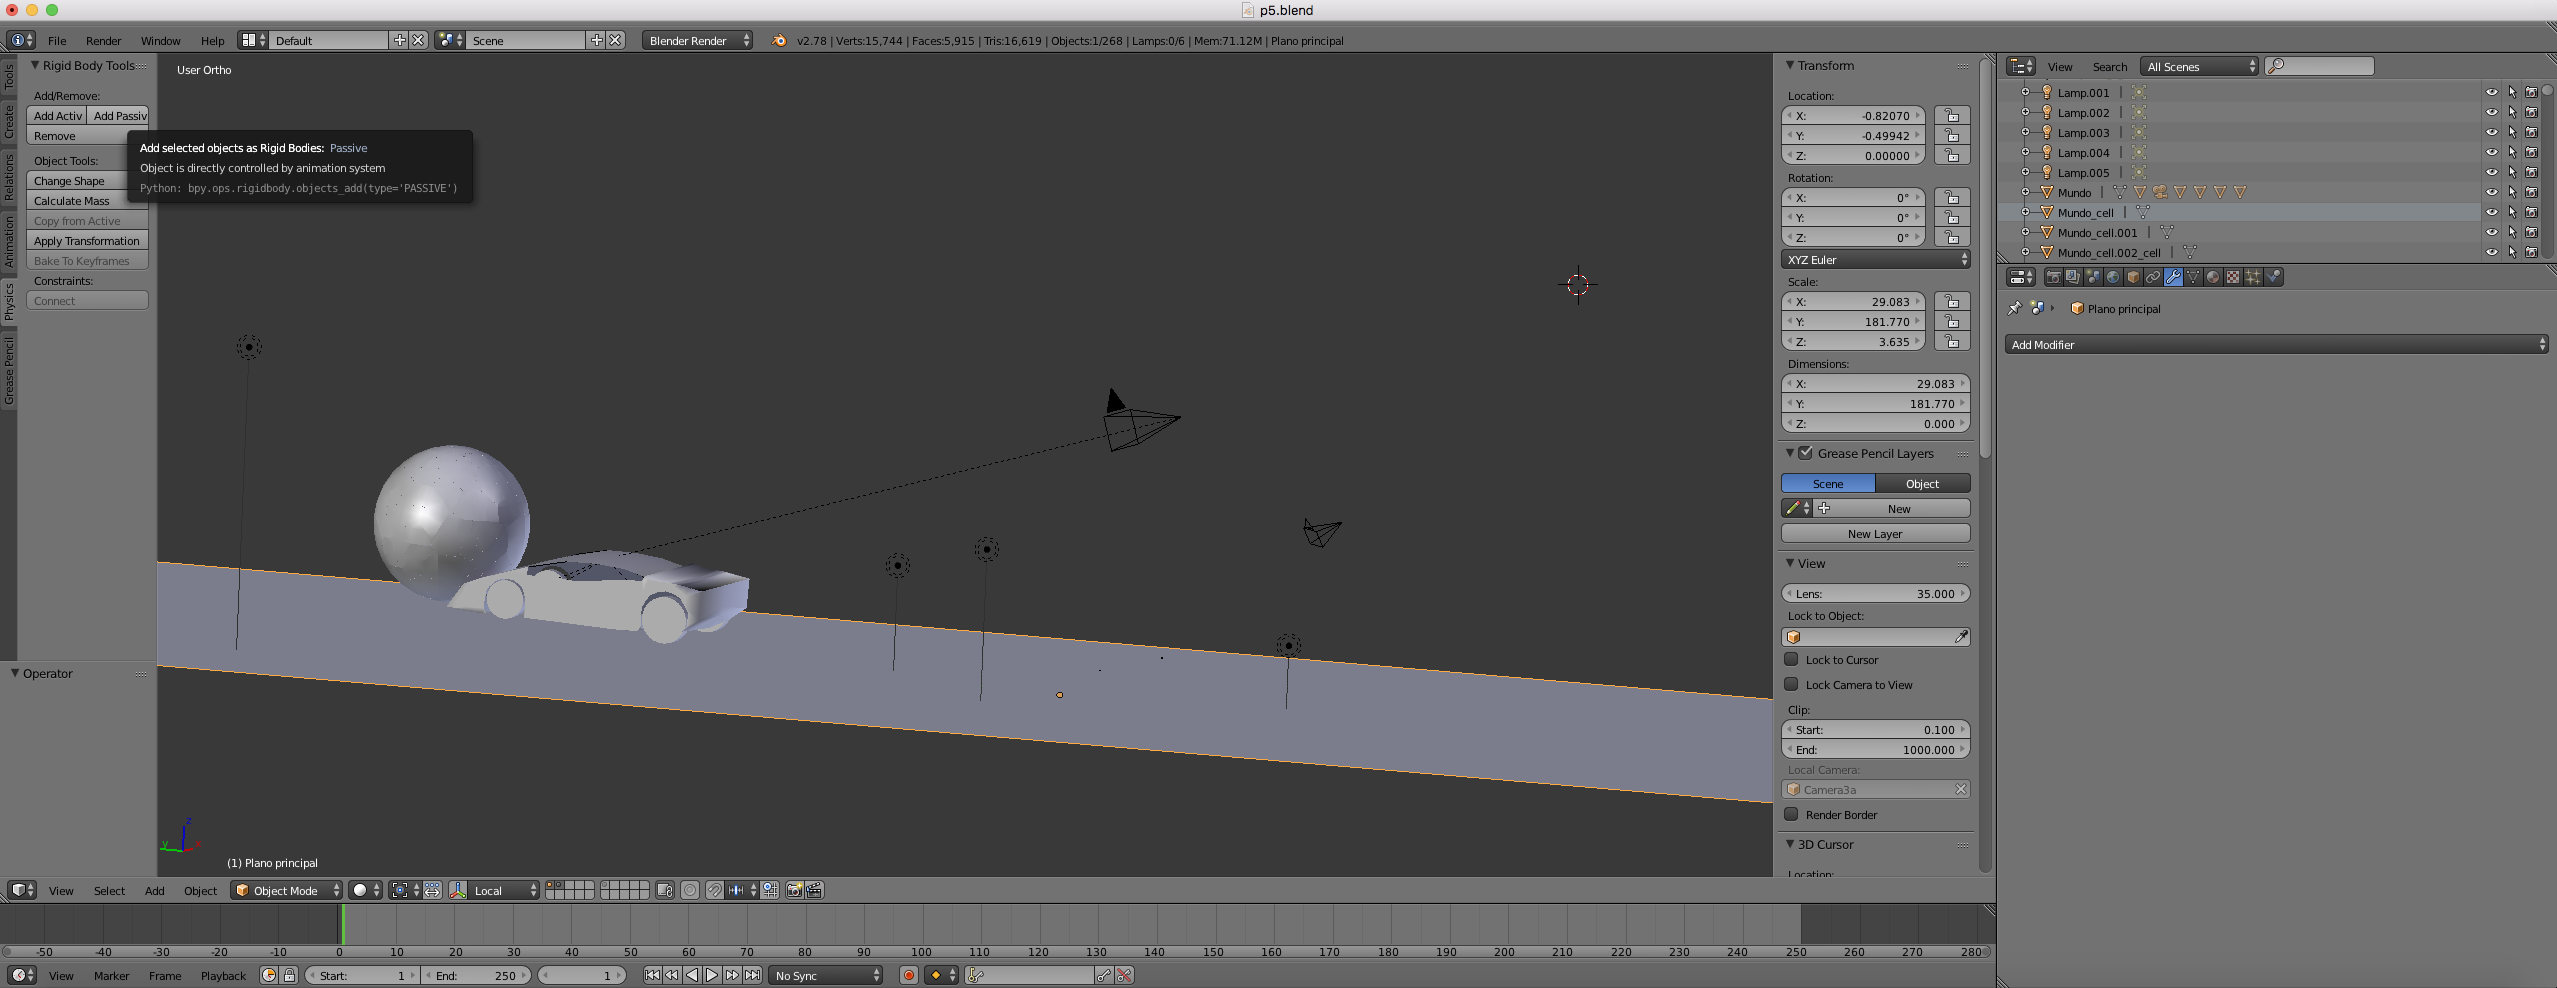
\includegraphics[width = 1.00\textwidth]{Imagenes/p5-img11}
 		\captionof{figure}{\label{fig:IPN}Estableciendo física pasiva al objeto ``Suelo''.}
	\end{center} 
\end{figure}

Con el objeto ``Coche'' seleccionado, vamos a añadir los fotogramas para establecer el tiempo de duración de la animación. La posición inicial será la que muestra en el escenario, por lo que pulsamos la tecla \textbf{I} y establecemos ese primer fotograma. Seguidamente ponemos el final de la animación en el fotograma 20 y volvemos a pulsar la tecla \textbf{I} como muestran las imágenes. \\

\begin{figure}[H]
	\begin{center}
	 		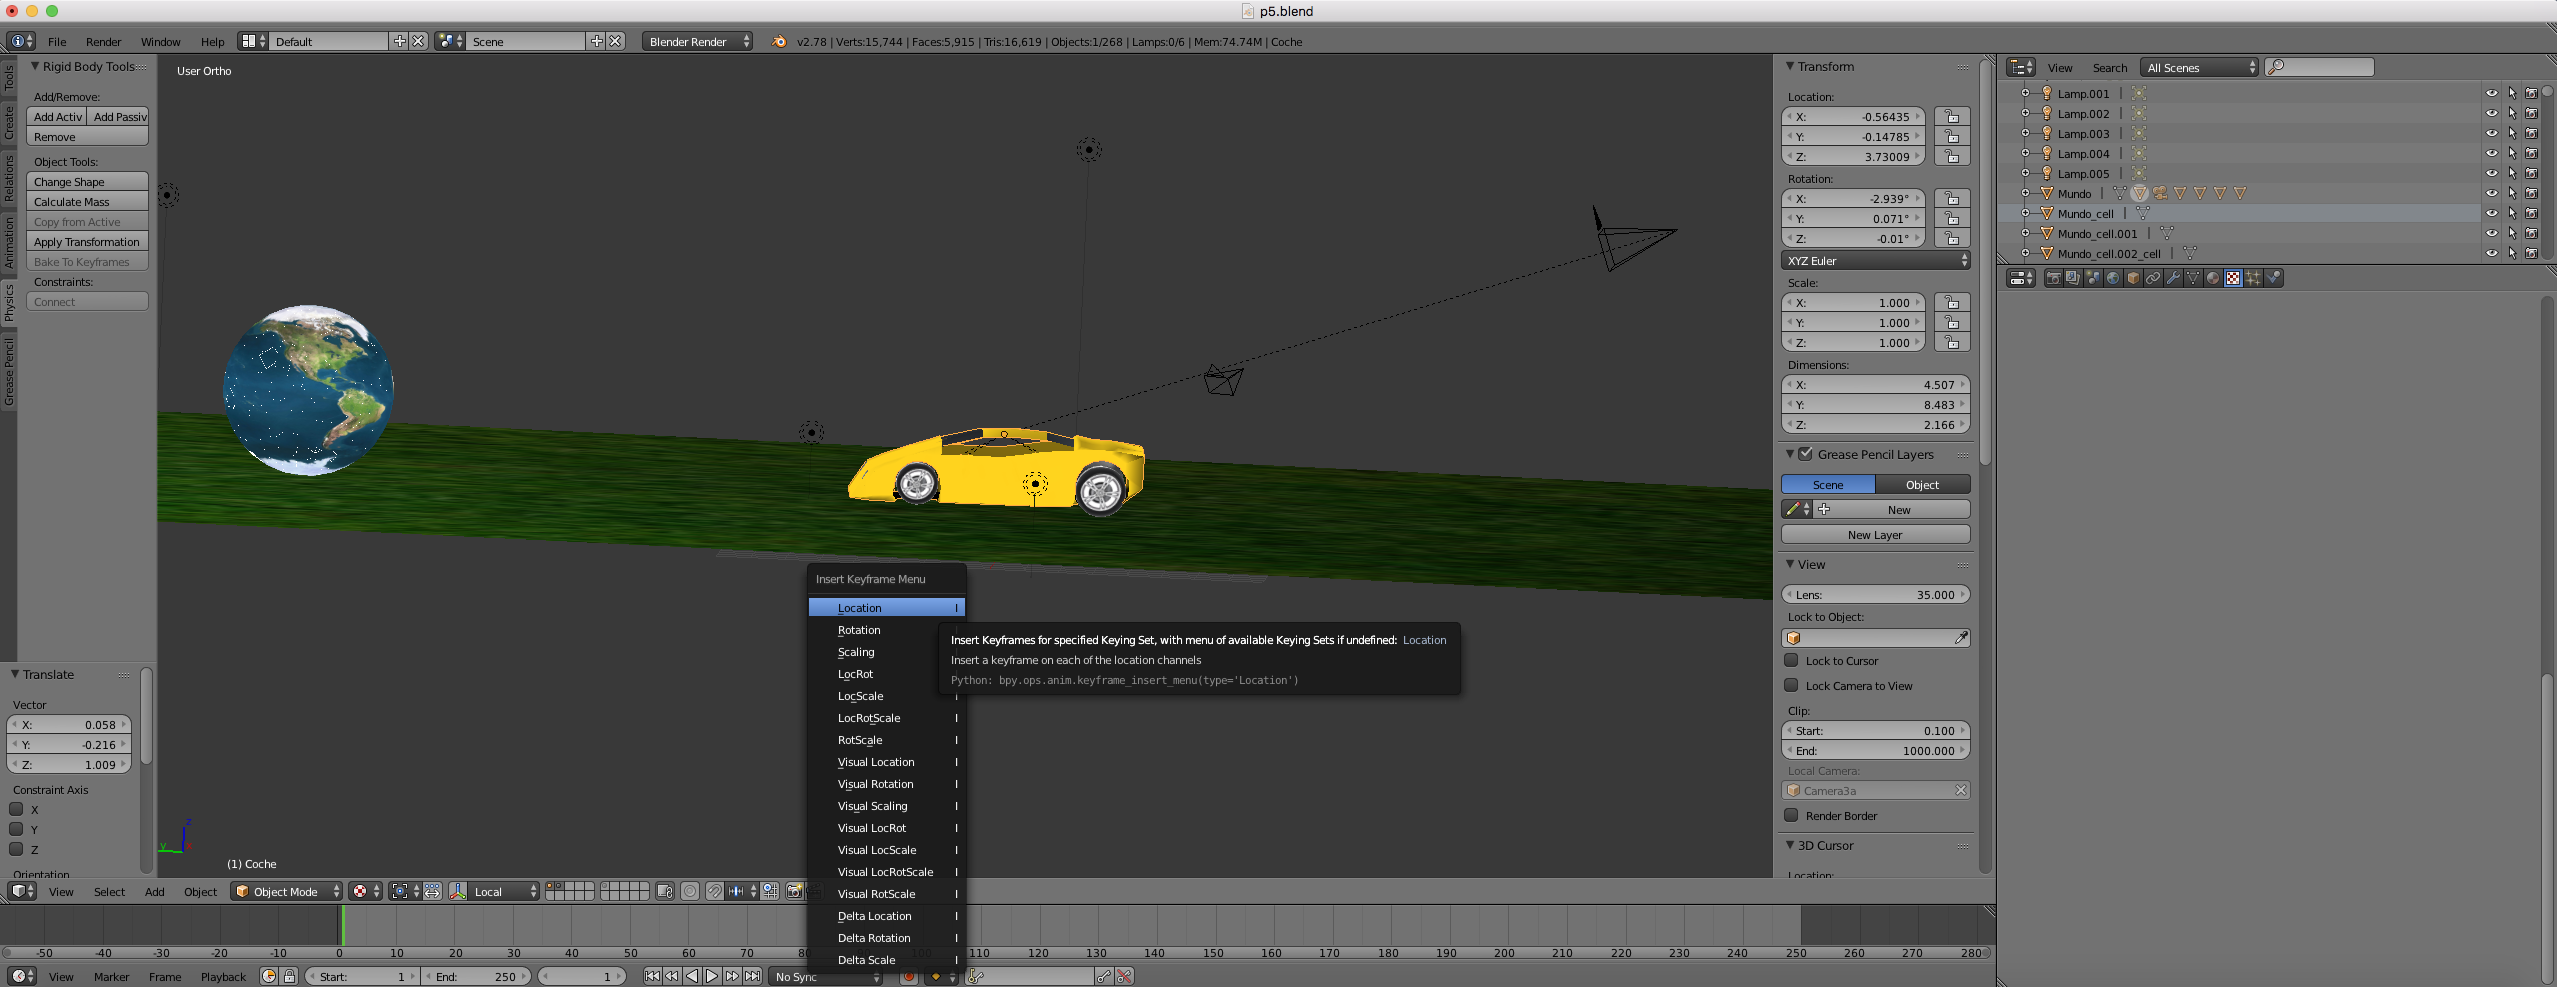
\includegraphics[width = 1.00\textwidth]{Imagenes/p5-img12}
 		\captionof{figure}{\label{fig:IPN}Estableciendo fotograma de inicio.}
	\end{center} 
\end{figure}

\begin{figure}[H]
	\begin{center}
	 		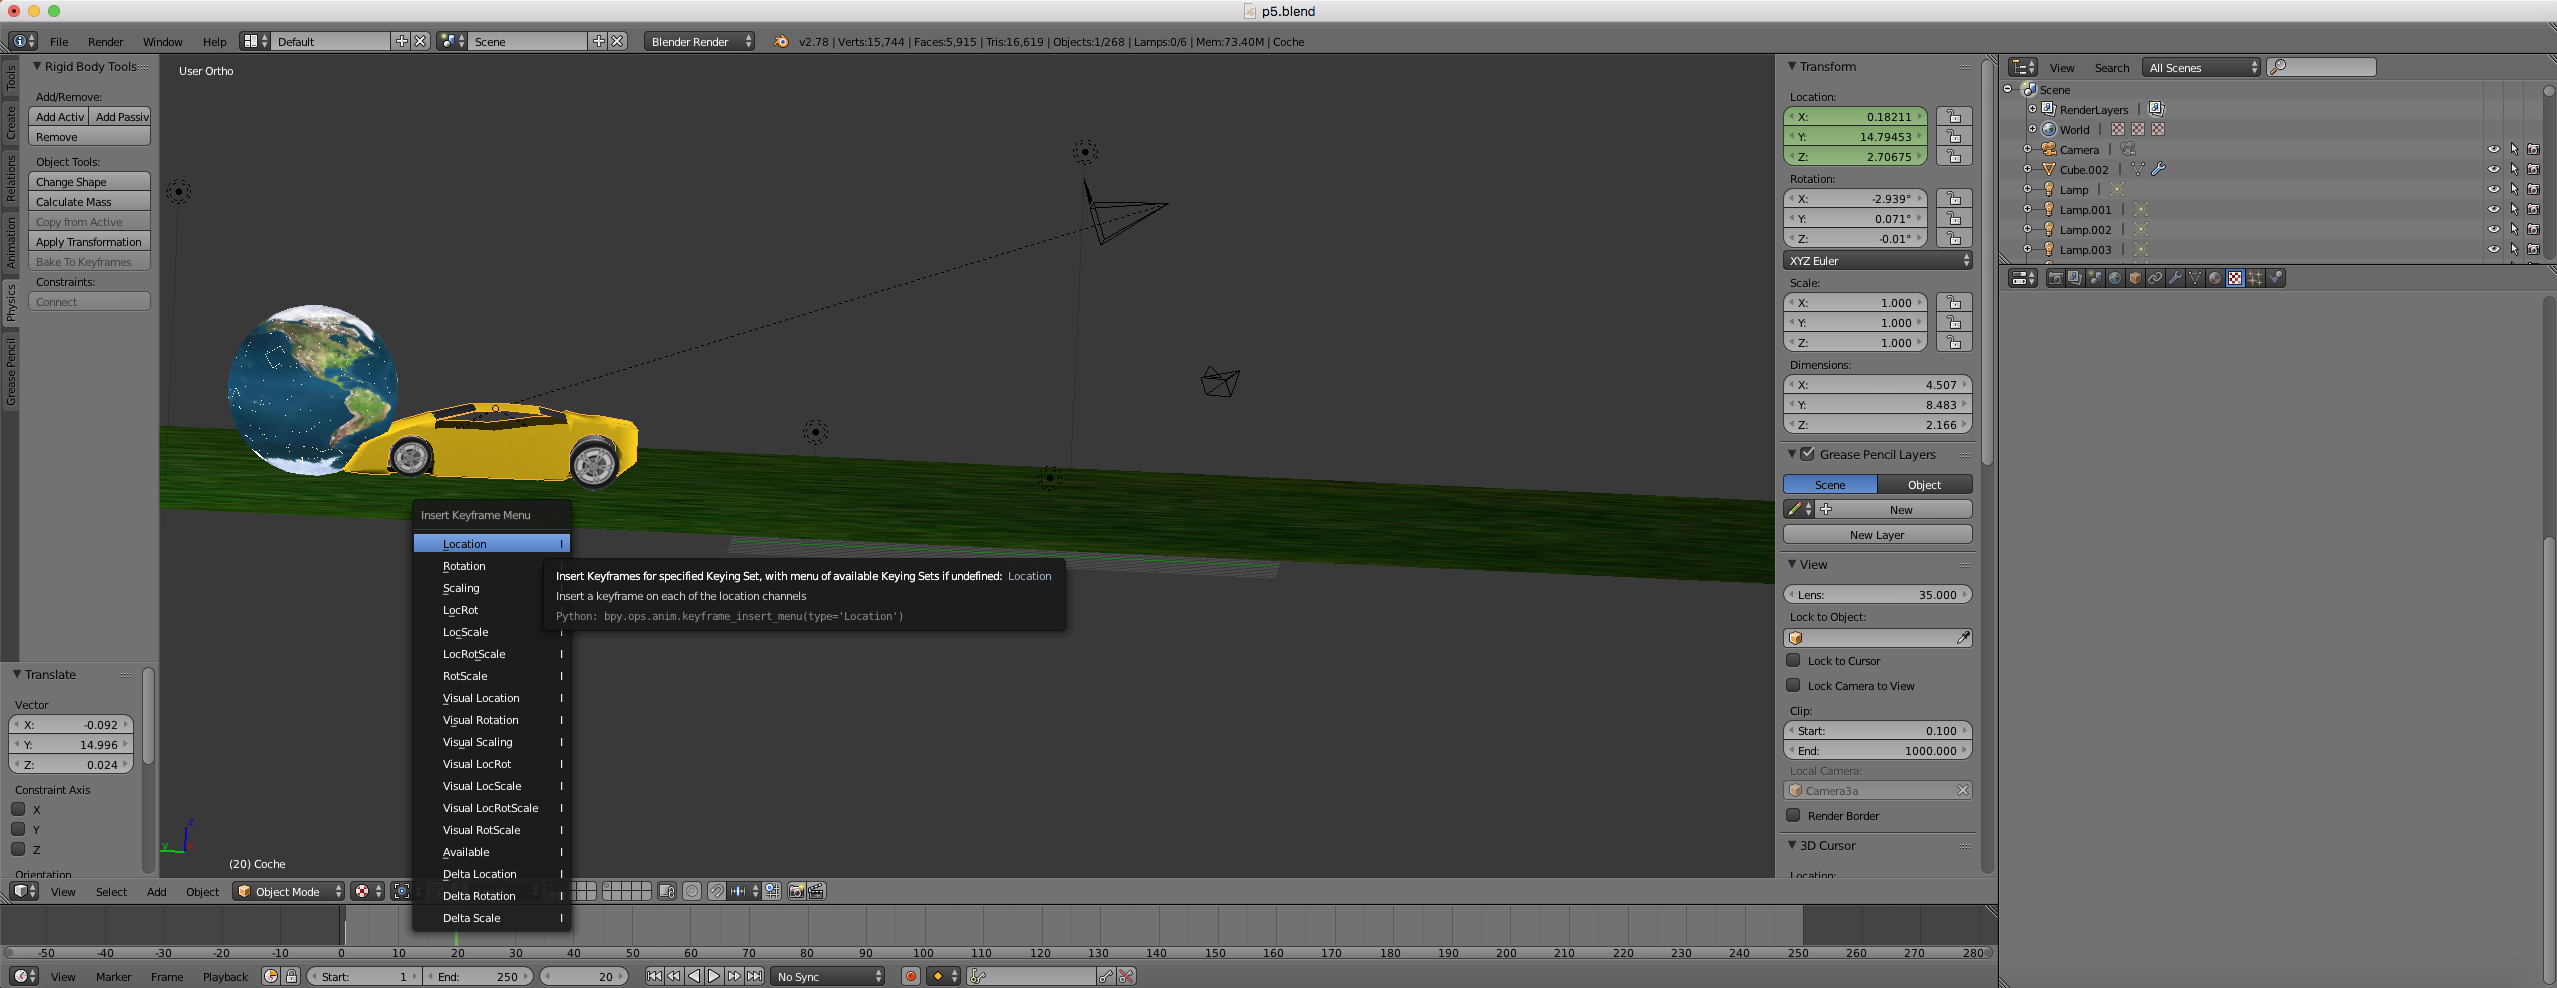
\includegraphics[width = 1.00\textwidth]{Imagenes/p5-img13}
 		\captionof{figure}{\label{fig:IPN}Estableciendo fotograma de fin.}
	\end{center} 
\end{figure}

Ahora es necesario ajustar una serie de parámetros para evitar que el objeto ``Mundo'' se desarme antes de que se produzca la colisión.  Con dicho objeto seleccionado, colocamos el inicio de la simulación en el fotograma 1, a continuación activamos las opciones \textbf{Enable Deactivation} y \textbf{Start Deactivated} en las propiedades físicas del objeto (habiendo previamente seleccionado todo el objeto pulsando la tecla \textbf{A}). En el panel \textbf{Physics} de la izquierda pulsamos la opción \textbf{Copy from Active} para que copie del activo. \\

\begin{figure}[H]
	\begin{center}
	 		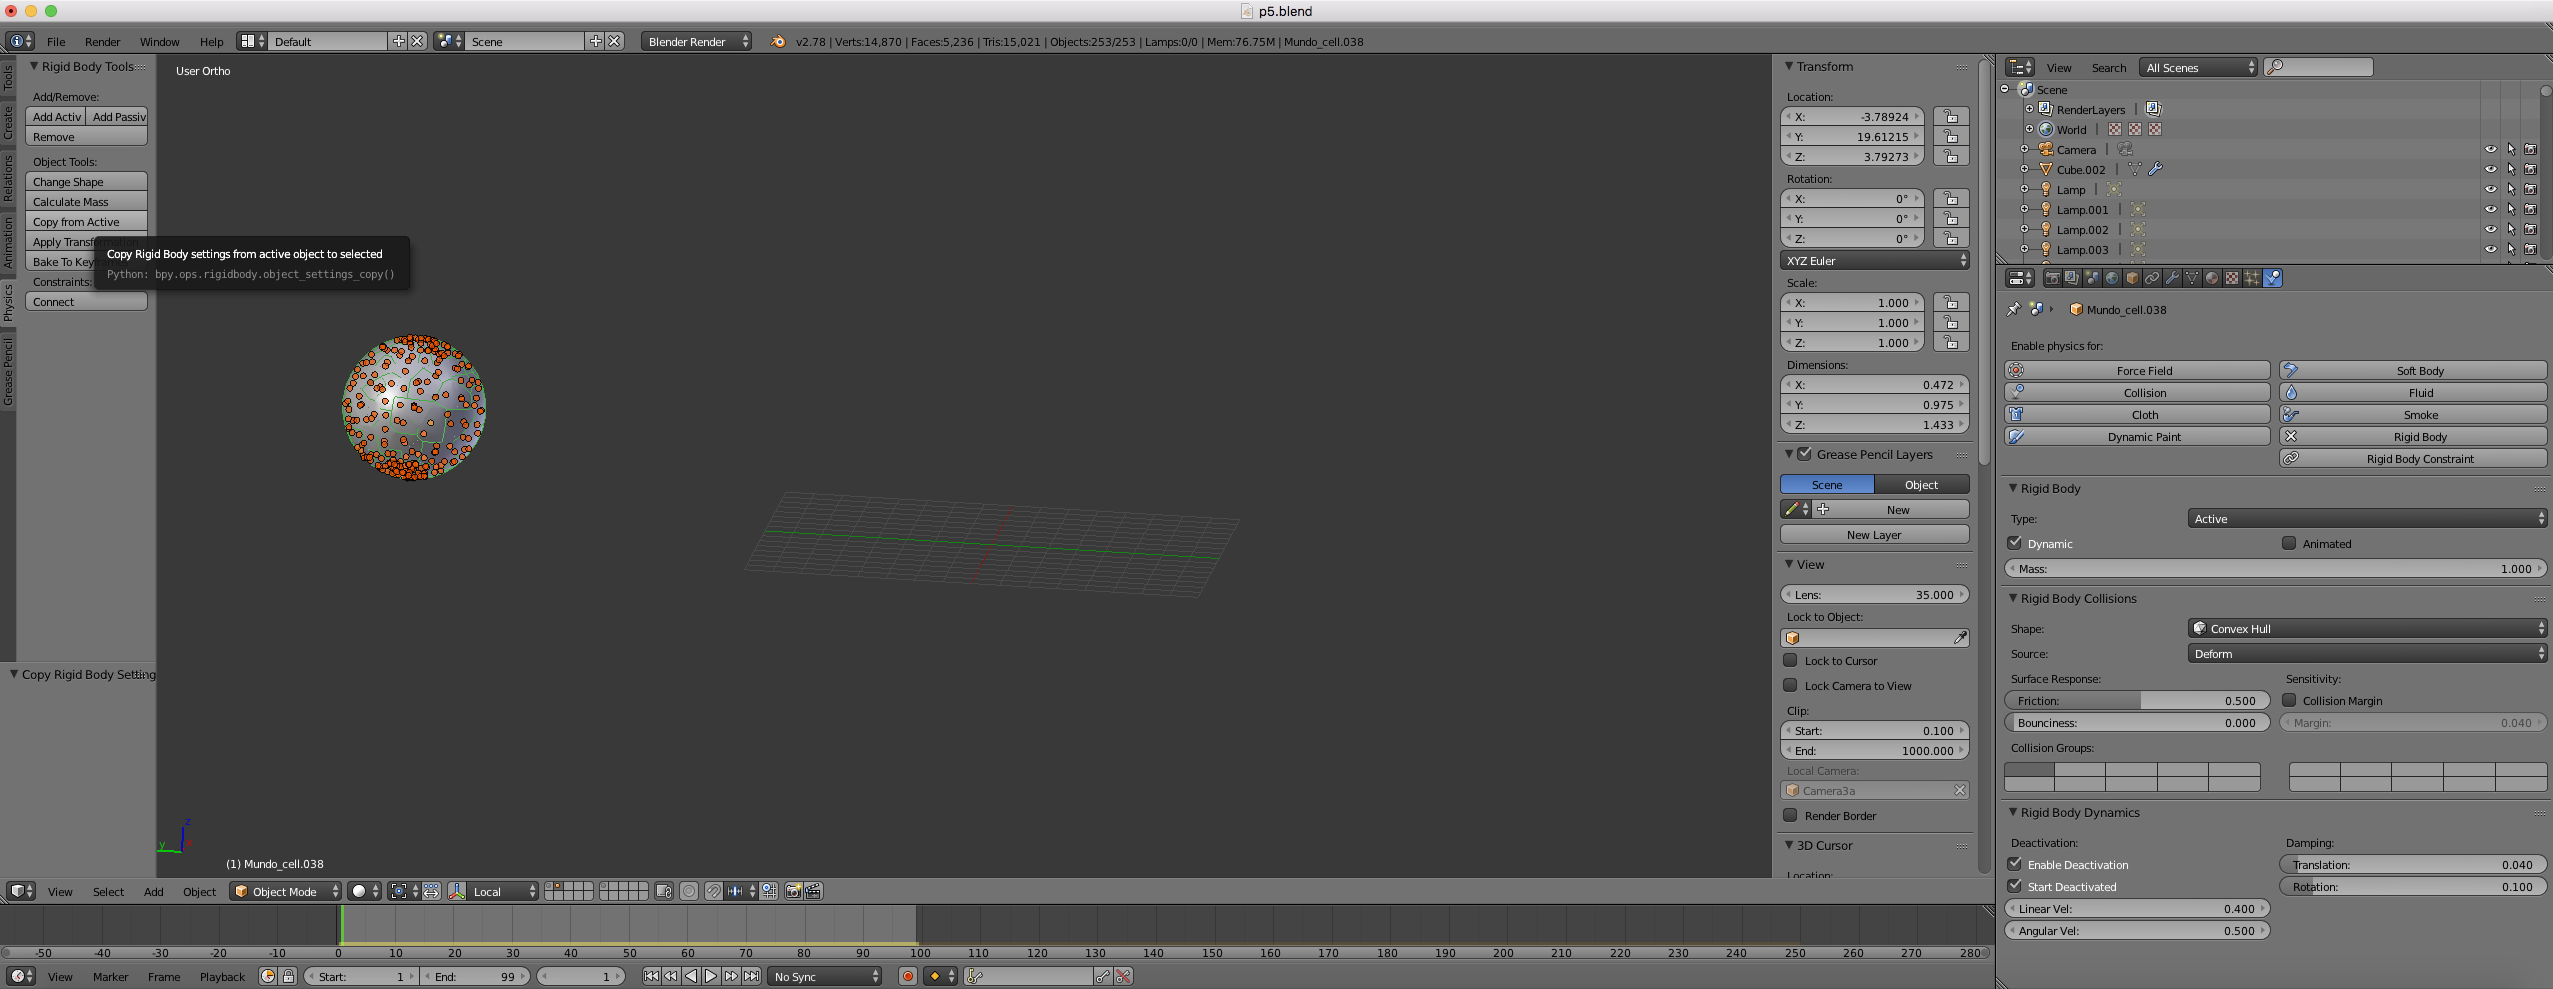
\includegraphics[width = 1.00\textwidth]{Imagenes/p5-img14}
 		\captionof{figure}{\label{fig:IPN}Estableciendo propiedades físicas al objeto ``Mundo''.}
	\end{center} 
\end{figure}

Situados en la misma capa seleccinamos el objeto ``Coche'' para activarle la opción \textbf{Add Active}. Nuevamente en las propiedades físicas, en este caso del objeto coche, activamos la opción \textbf{Animated}. Con el puntero colocado encima de esa opción pulsamos la tecla \textbf{I} para darle un fotograma y lo mismo hacemos pero poniendo el fotograma en 20. En el fotograma 21 descativamos dicha opción y volvemos a pulsar la tecla \textbf{I}. También subimos la masa del objeto a 50\\

\begin{figure}[H]
	\begin{center}
	 		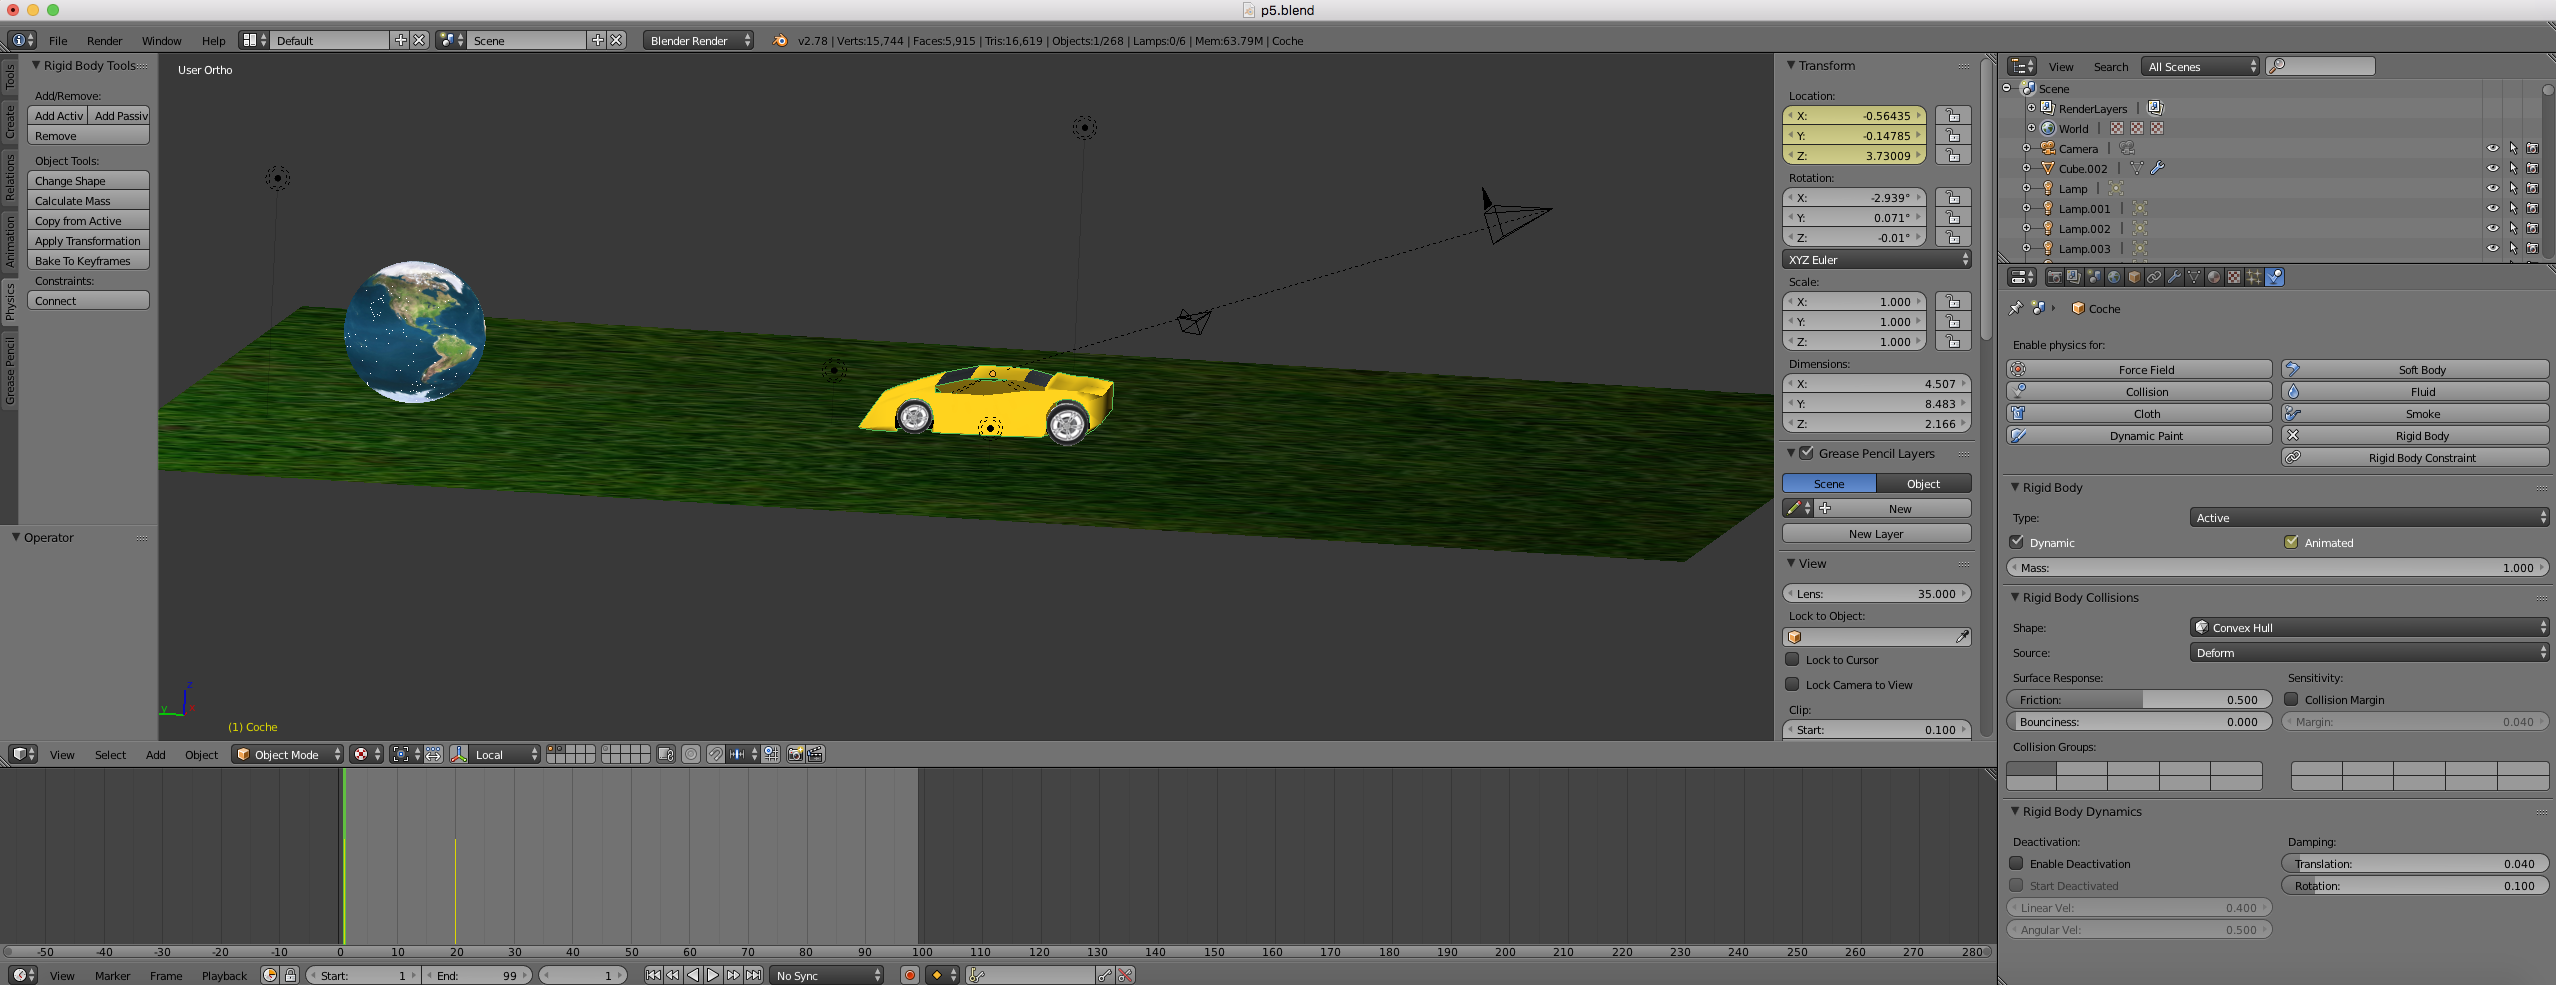
\includegraphics[width = 1.00\textwidth]{Imagenes/p5-img15}
 		\captionof{figure}{\label{fig:IPN}Estableciendo propiedades físicas al objeto ``Coche'' (I).}
	\end{center} 
\end{figure}

\begin{figure}[H]
	\begin{center}
	 		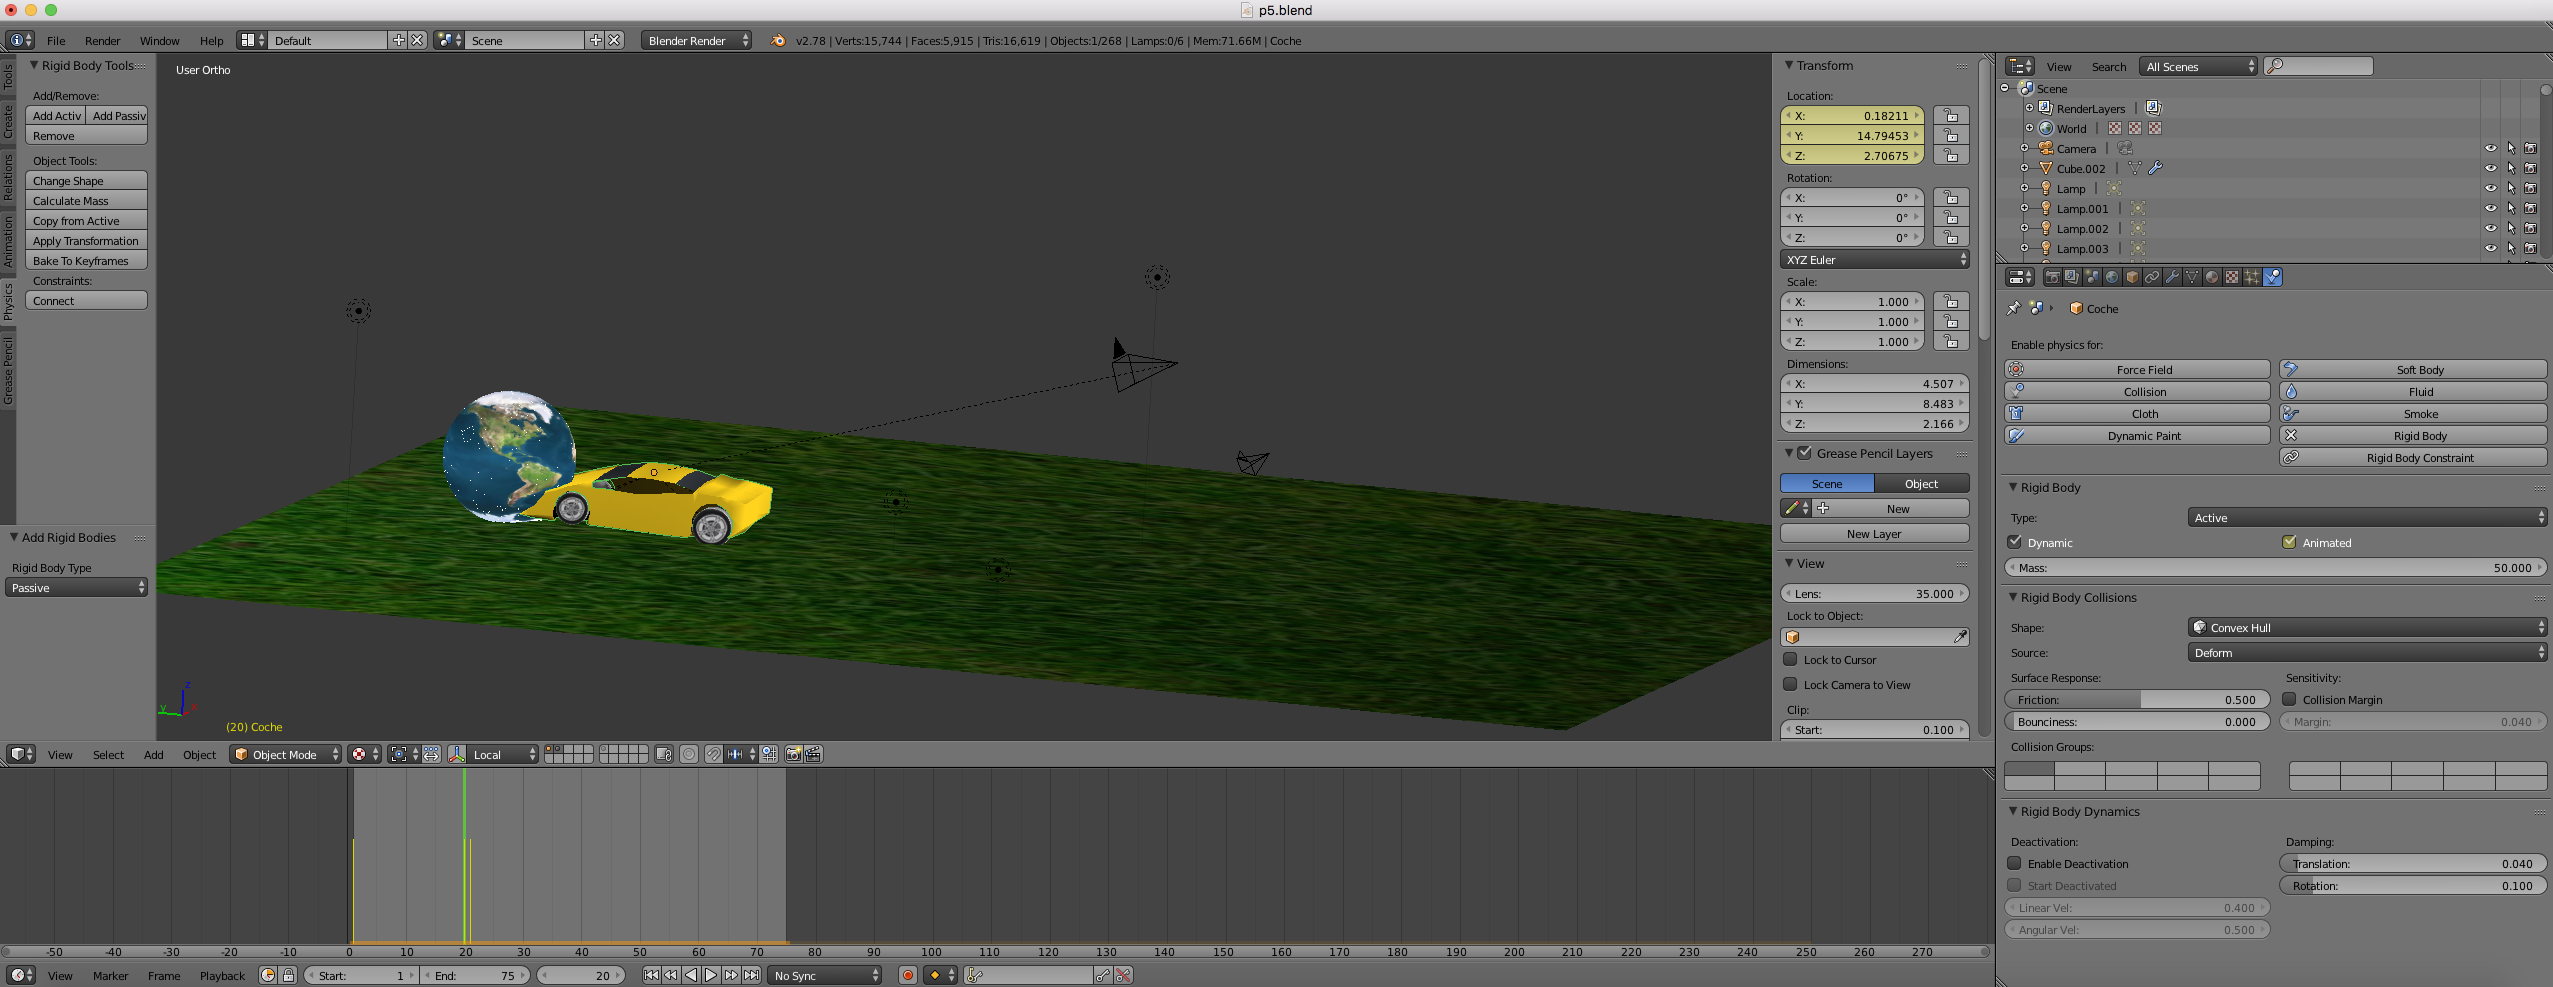
\includegraphics[width = 1.00\textwidth]{Imagenes/p5-img16}
 		\captionof{figure}{\label{fig:IPN}Estableciendo propiedades físicas al objeto ``Coche'' (II).}
	\end{center} 
\end{figure}

\begin{figure}[H]
	\begin{center}
	 		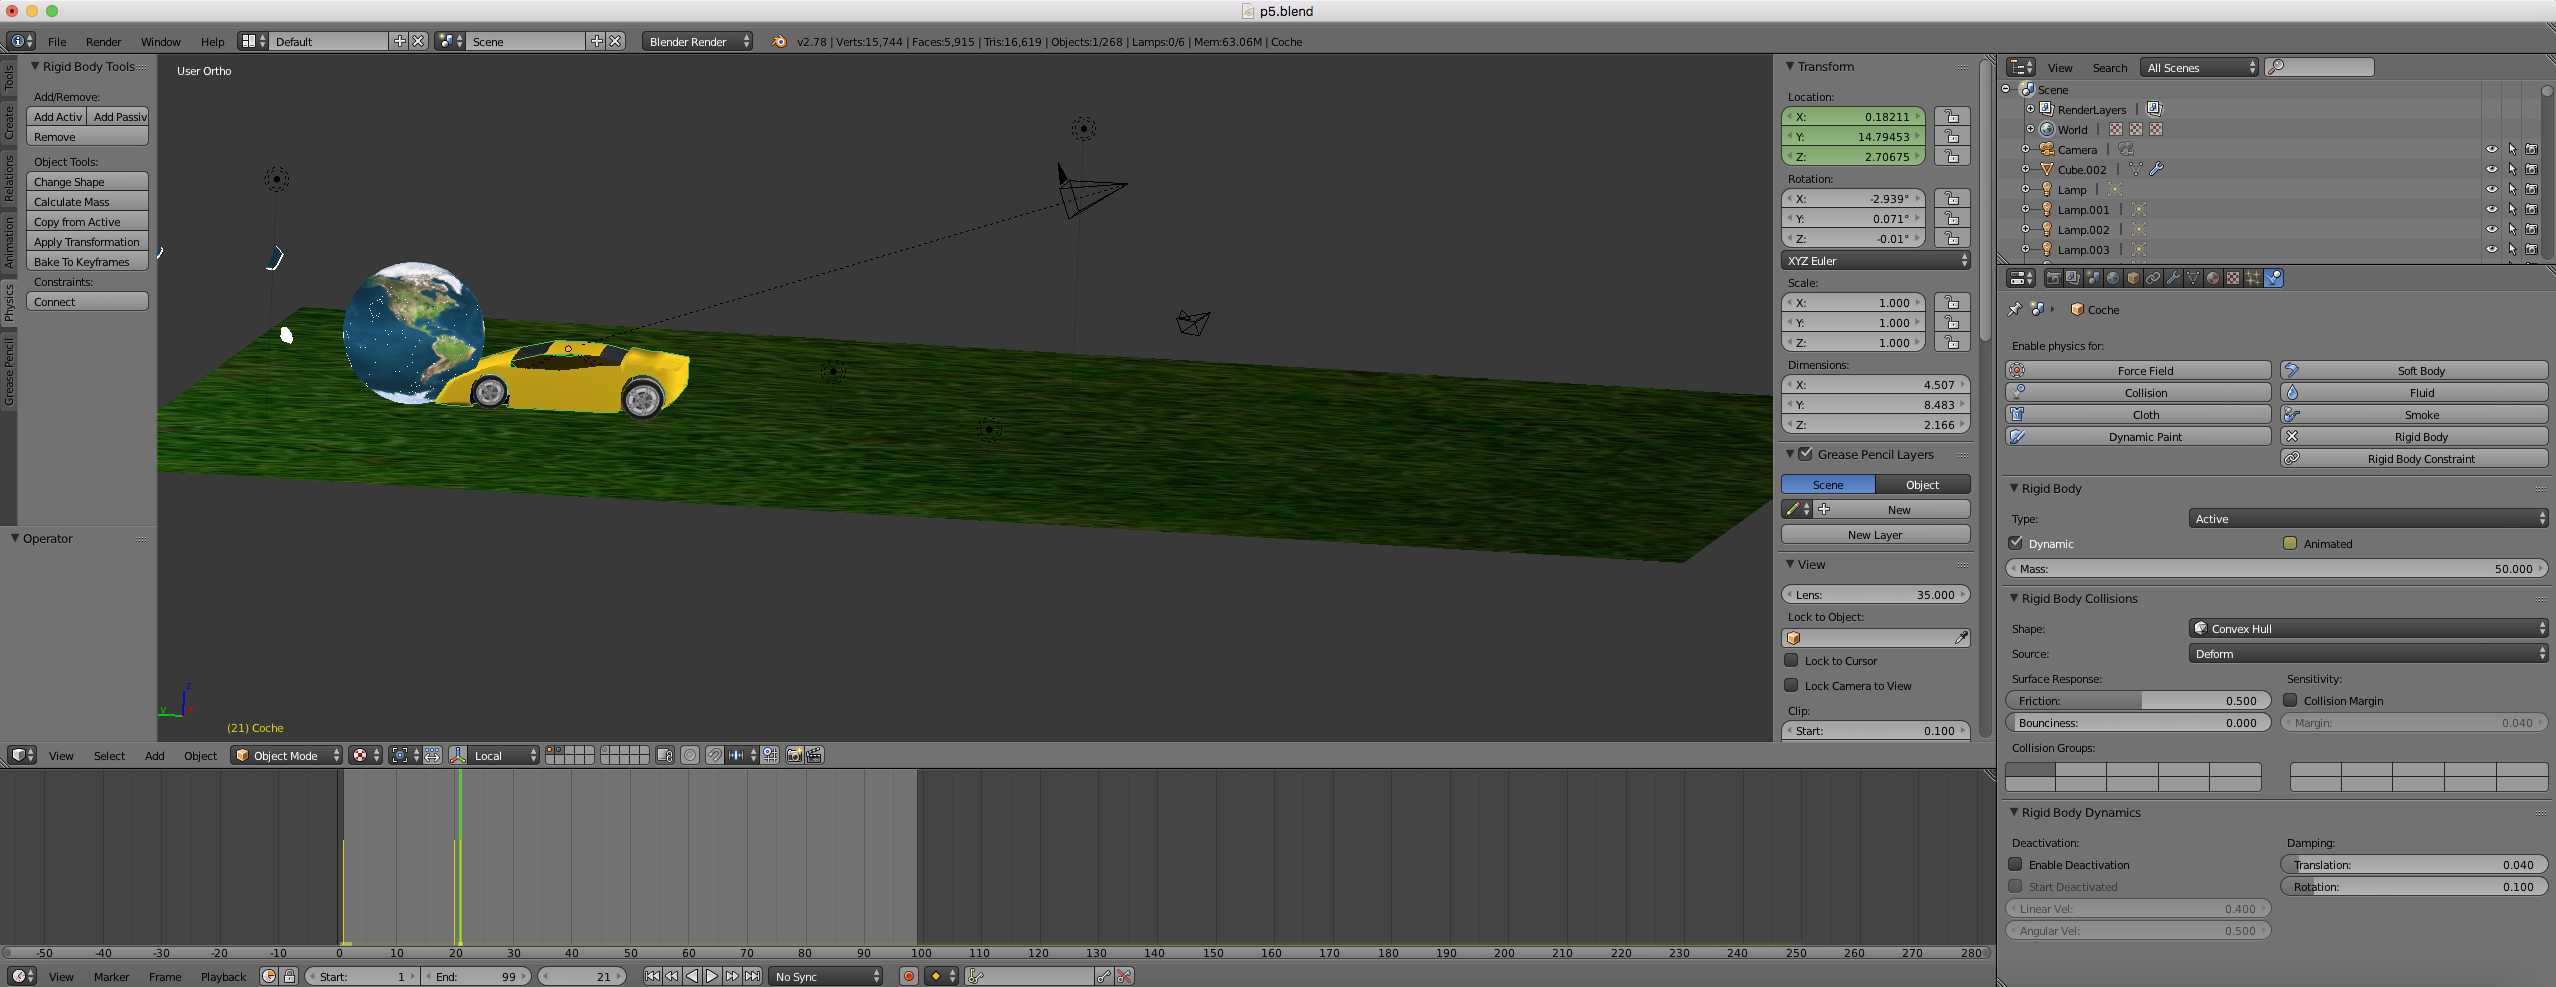
\includegraphics[width = 1.00\textwidth]{Imagenes/p5-img17}
 		\captionof{figure}{\label{fig:IPN}Estableciendo propiedades físicas al objeto ``Coche'' (III).}
	\end{center} 
\end{figure}

Con todo esto ya podemos ejecutar la simulación para comprobar que funciona correctamente y que el objeto ``Mundo'' se desarma cuando se produce la colisión con el objeto ``Coche'' dándole al botón de inicio correspondiente.\\

\begin{figure}[H]
	\begin{center}
	 		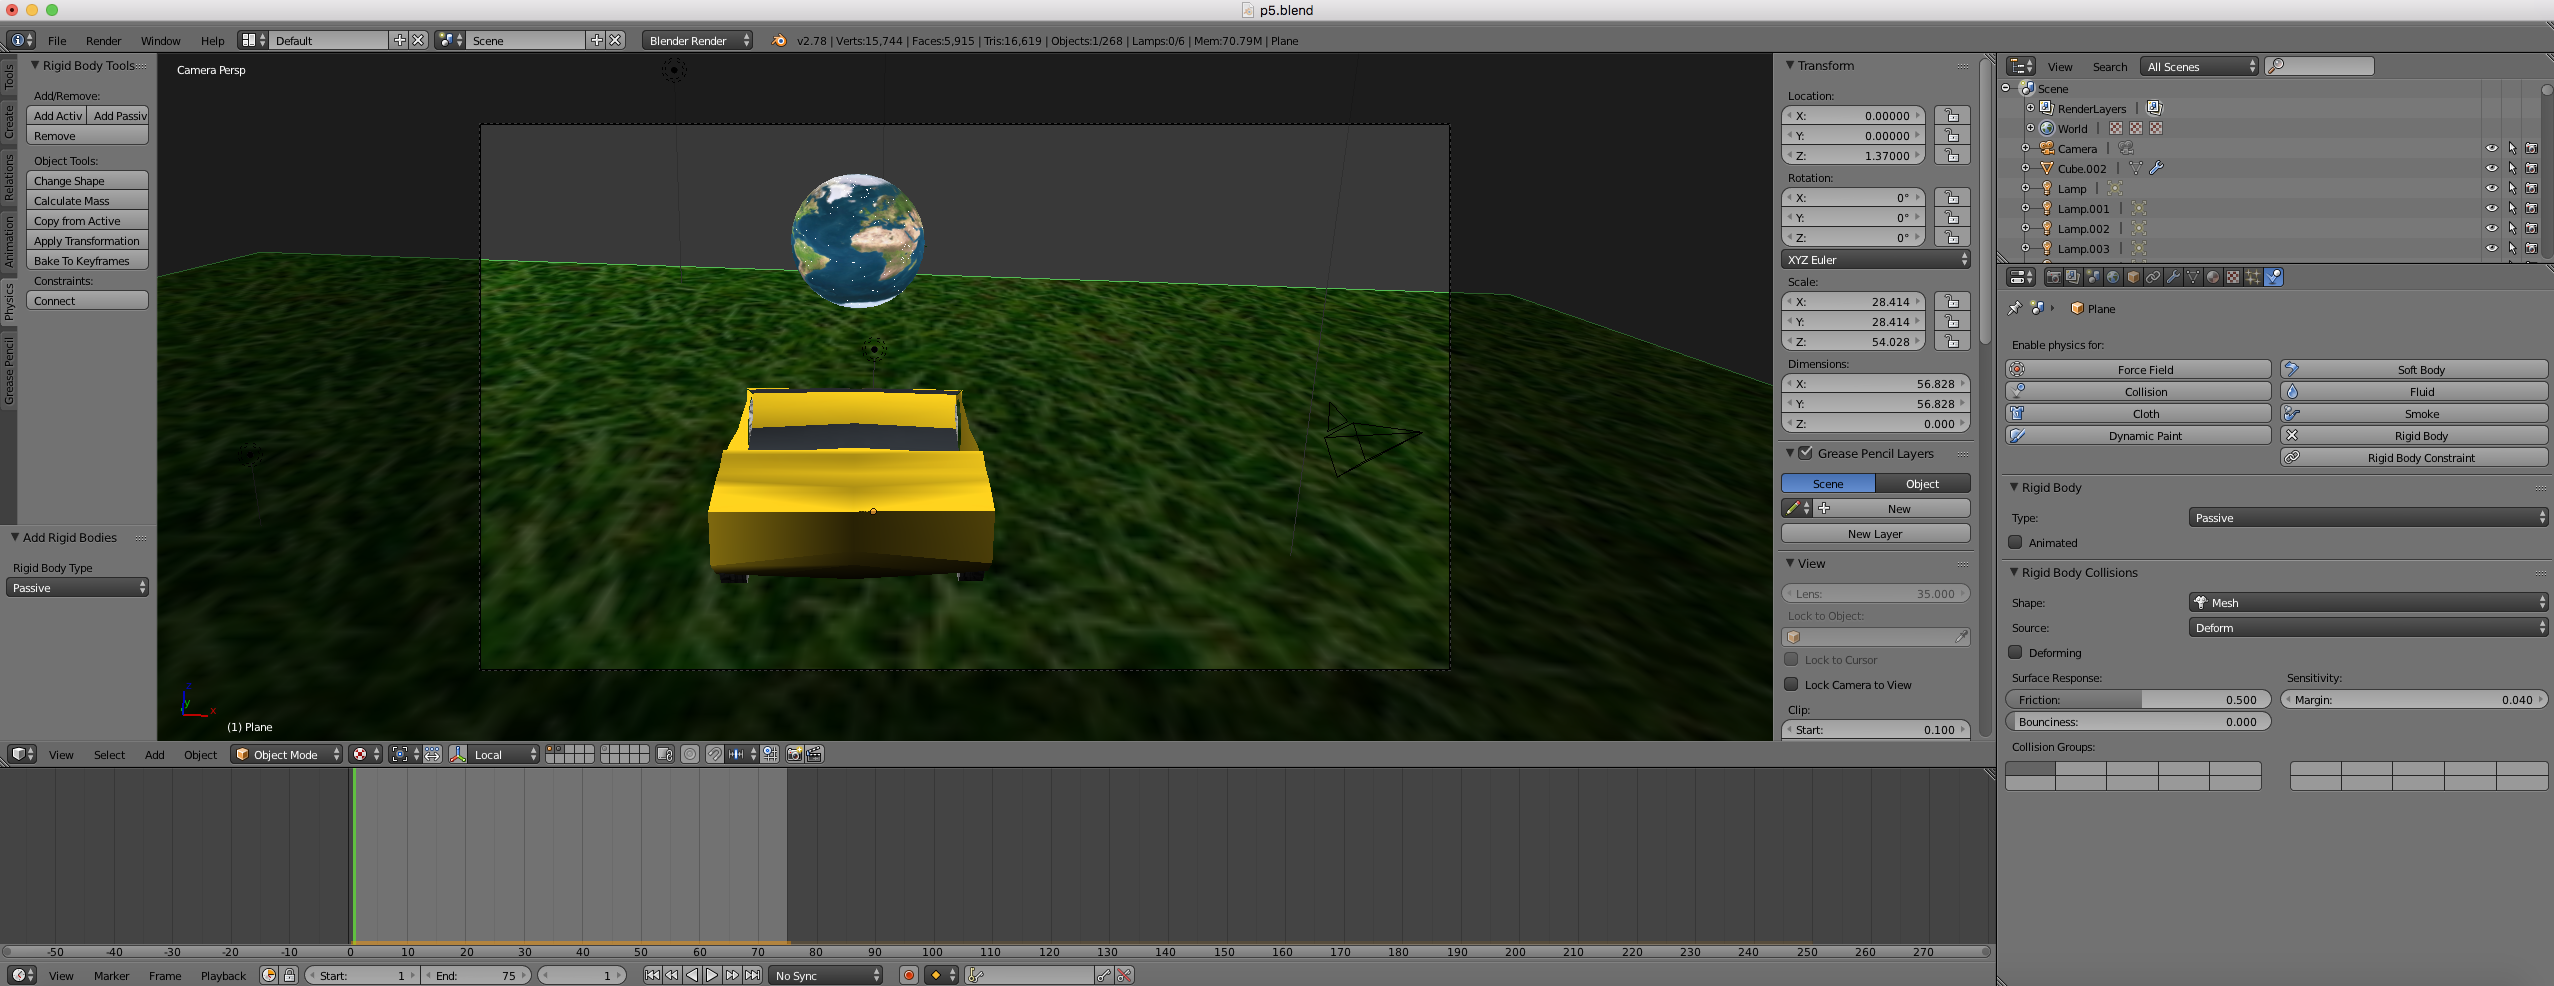
\includegraphics[width = 1.00\textwidth]{Imagenes/p5-img18}
 		\captionof{figure}{\label{fig:IPN}Simulando colisión (I).}
	\end{center} 
\end{figure}

\begin{figure}[H]
	\begin{center}
	 		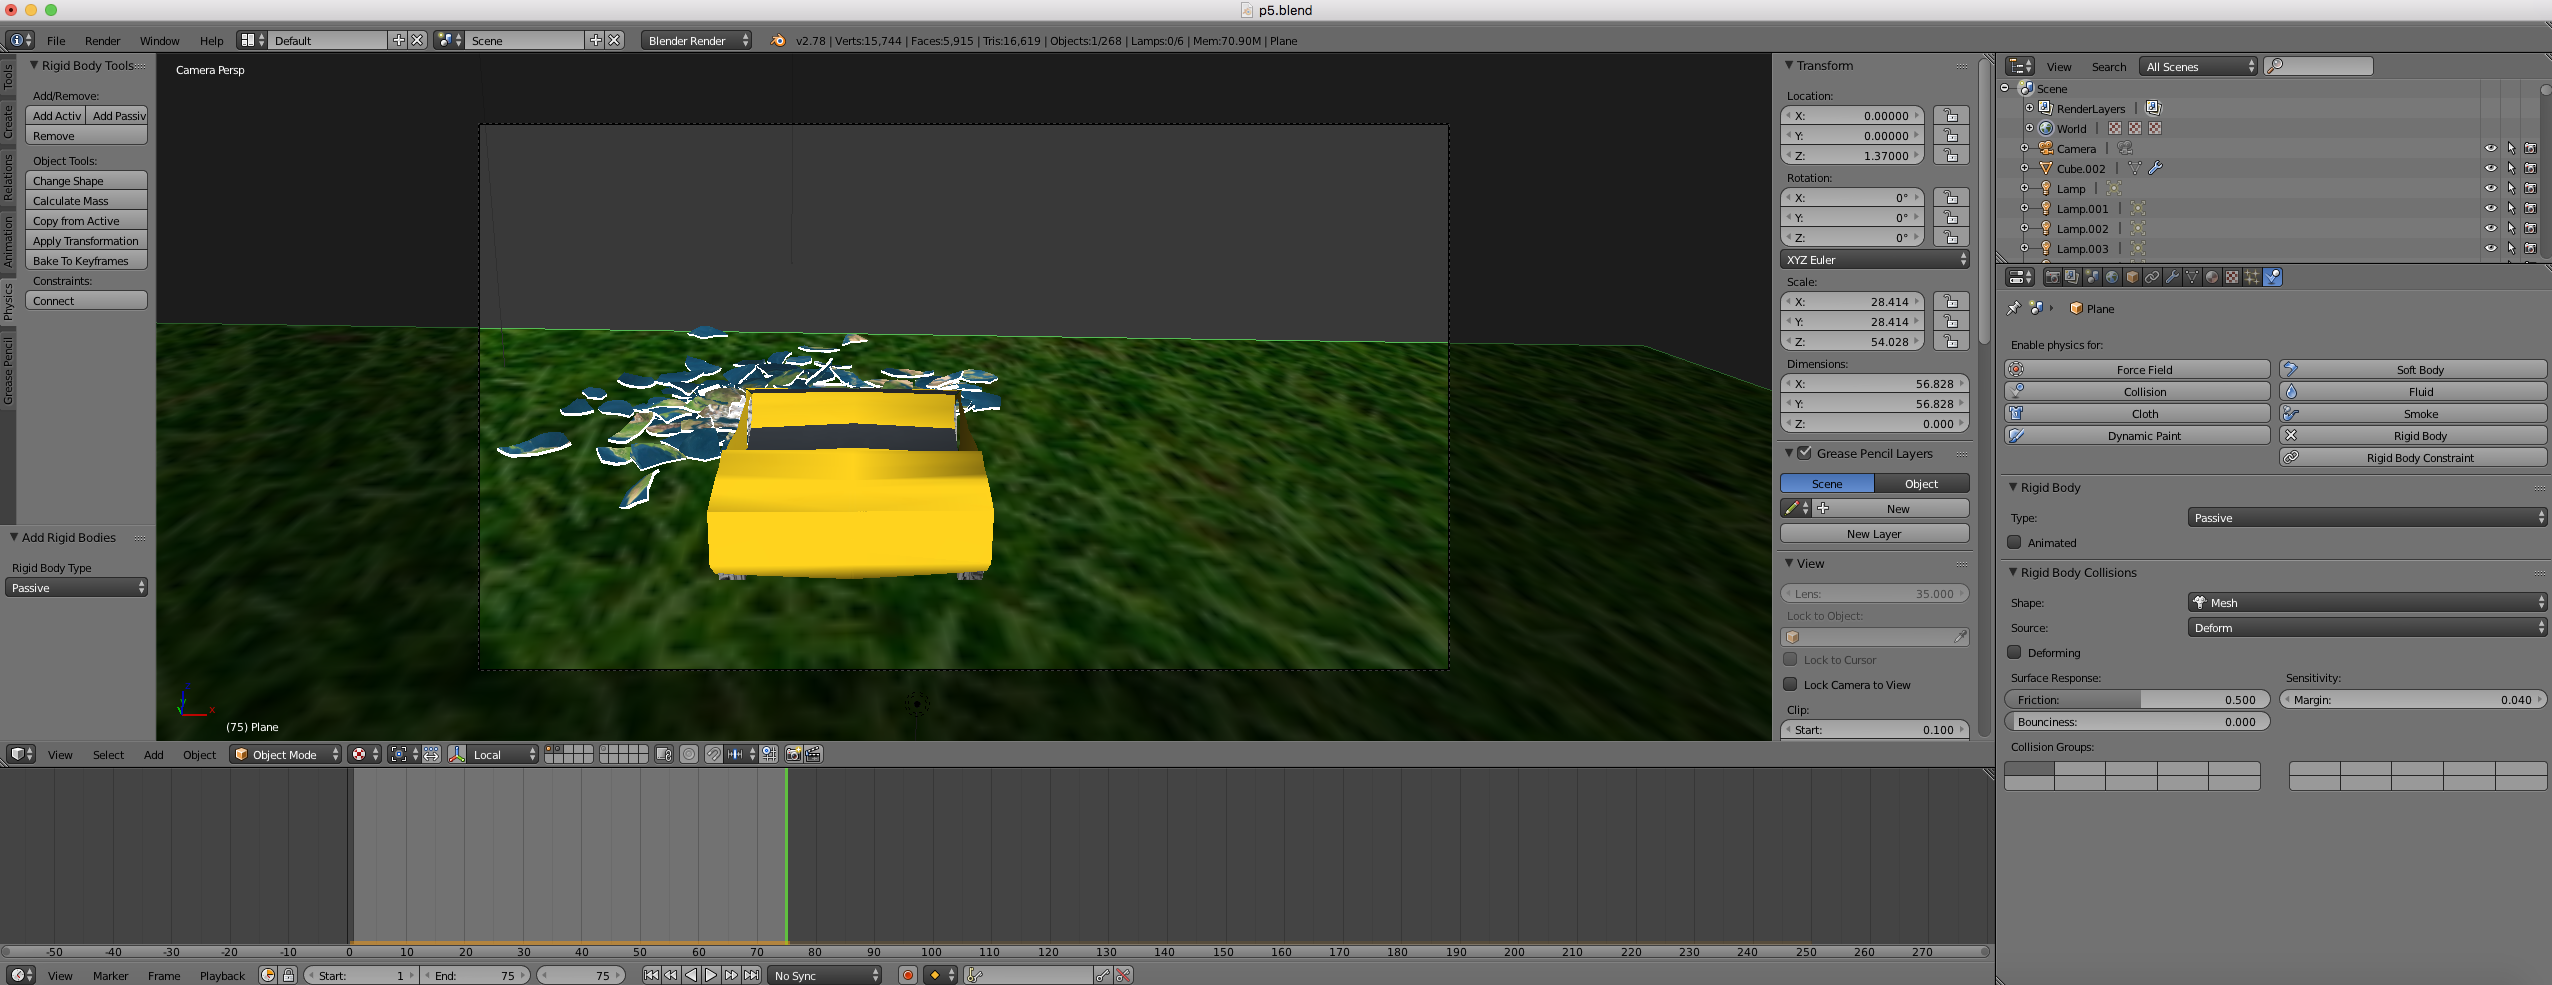
\includegraphics[width = 1.00\textwidth]{Imagenes/p5-img19}
 		\captionof{figure}{\label{fig:IPN}Simulando colisión (II).}
	\end{center} 
\end{figure}

\begin{figure}[H]
	\begin{center}
	 		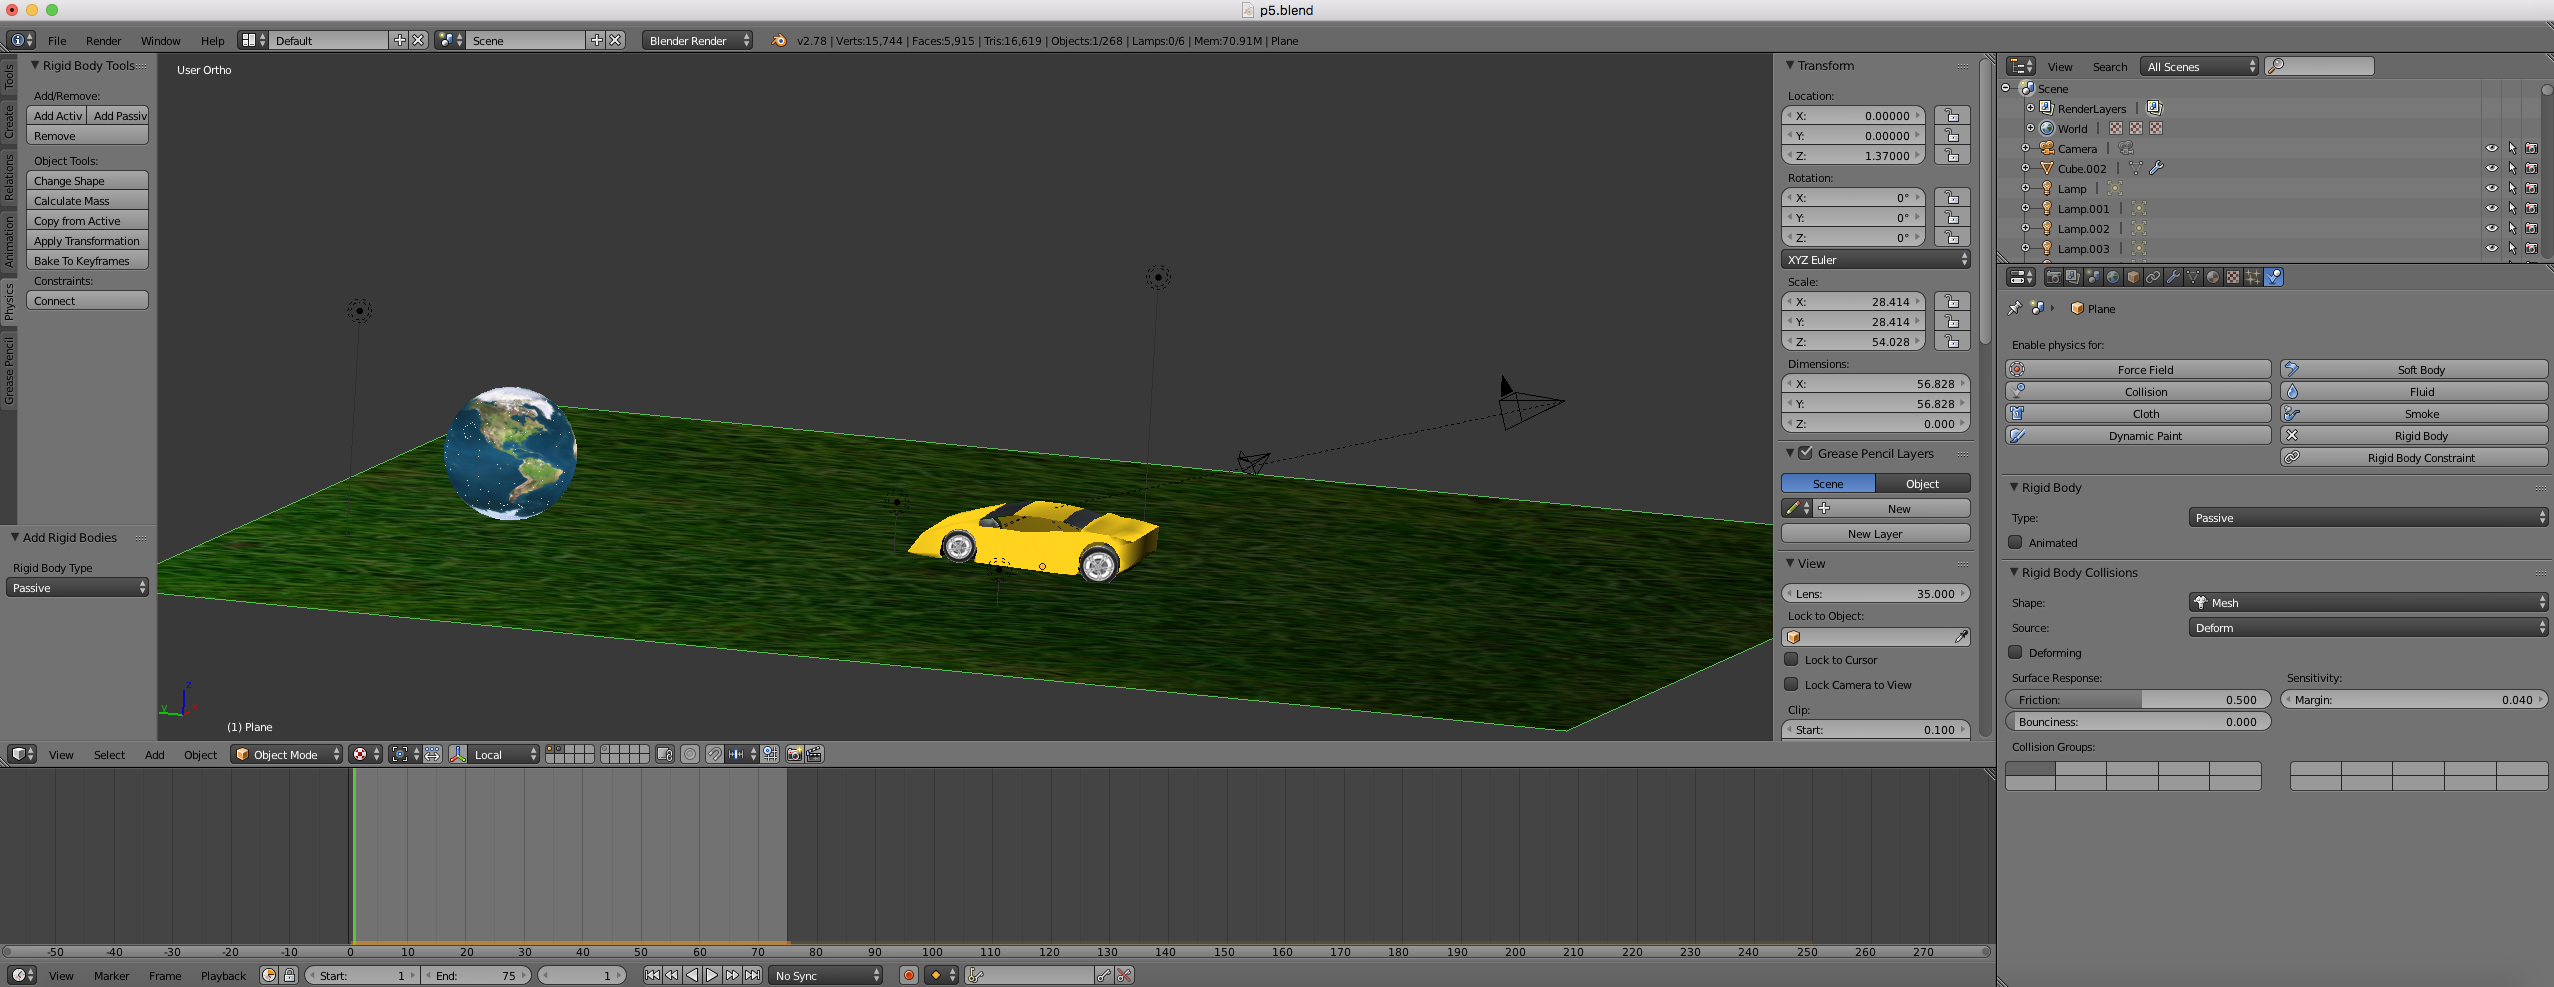
\includegraphics[width = 1.00\textwidth]{Imagenes/p5-img20}
 		\captionof{figure}{\label{fig:IPN}Simulando colisión (III).}
	\end{center} 
\end{figure}

\begin{figure}[H]
	\begin{center}
	 		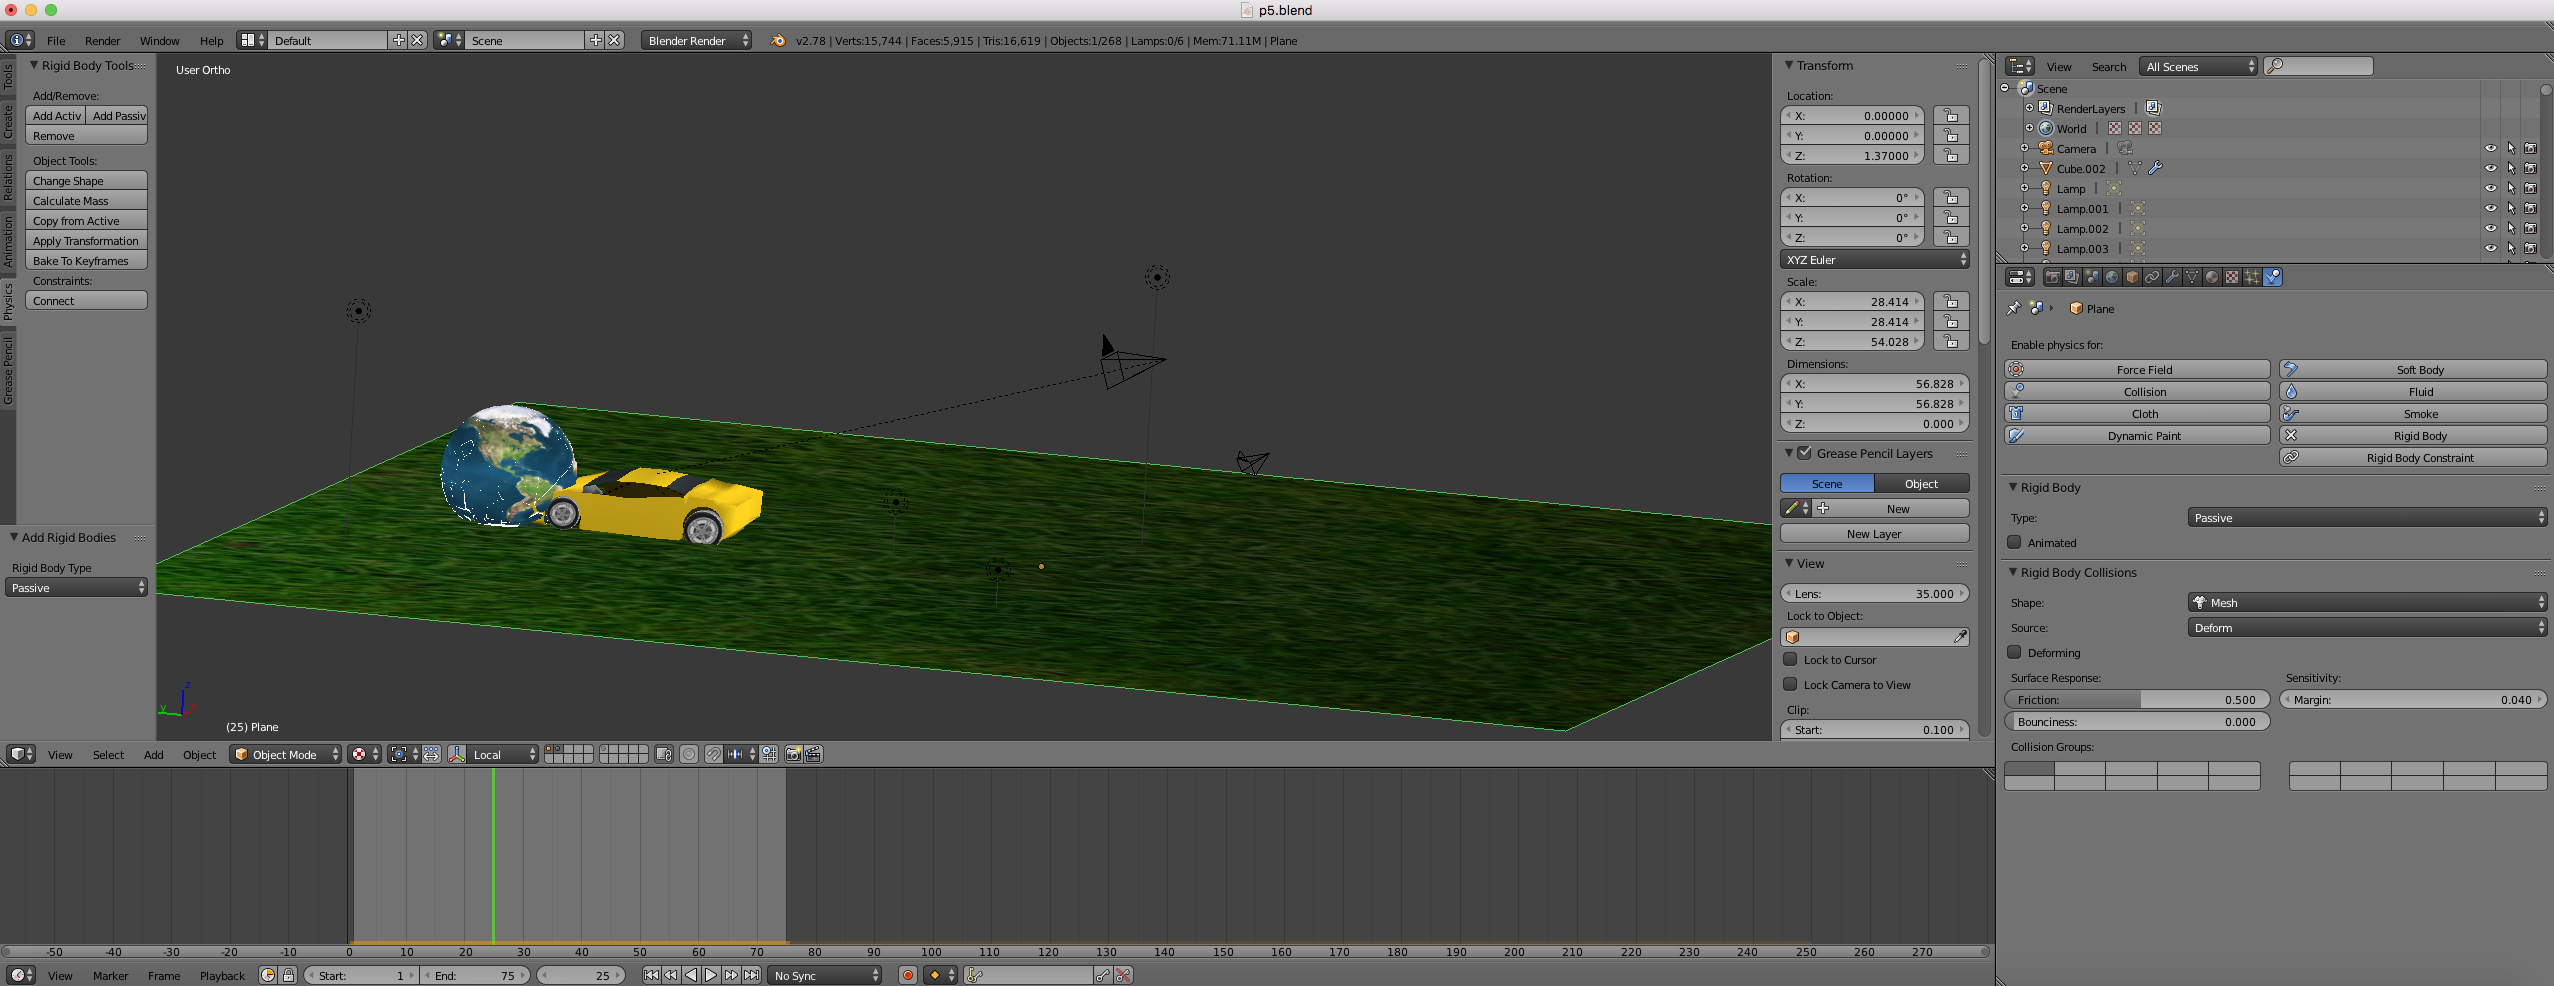
\includegraphics[width = 1.00\textwidth]{Imagenes/p5-img21}
 		\captionof{figure}{\label{fig:IPN}Simulando colisión (IV).}
	\end{center} 
\end{figure}

\begin{figure}[H]
	\begin{center}
	 		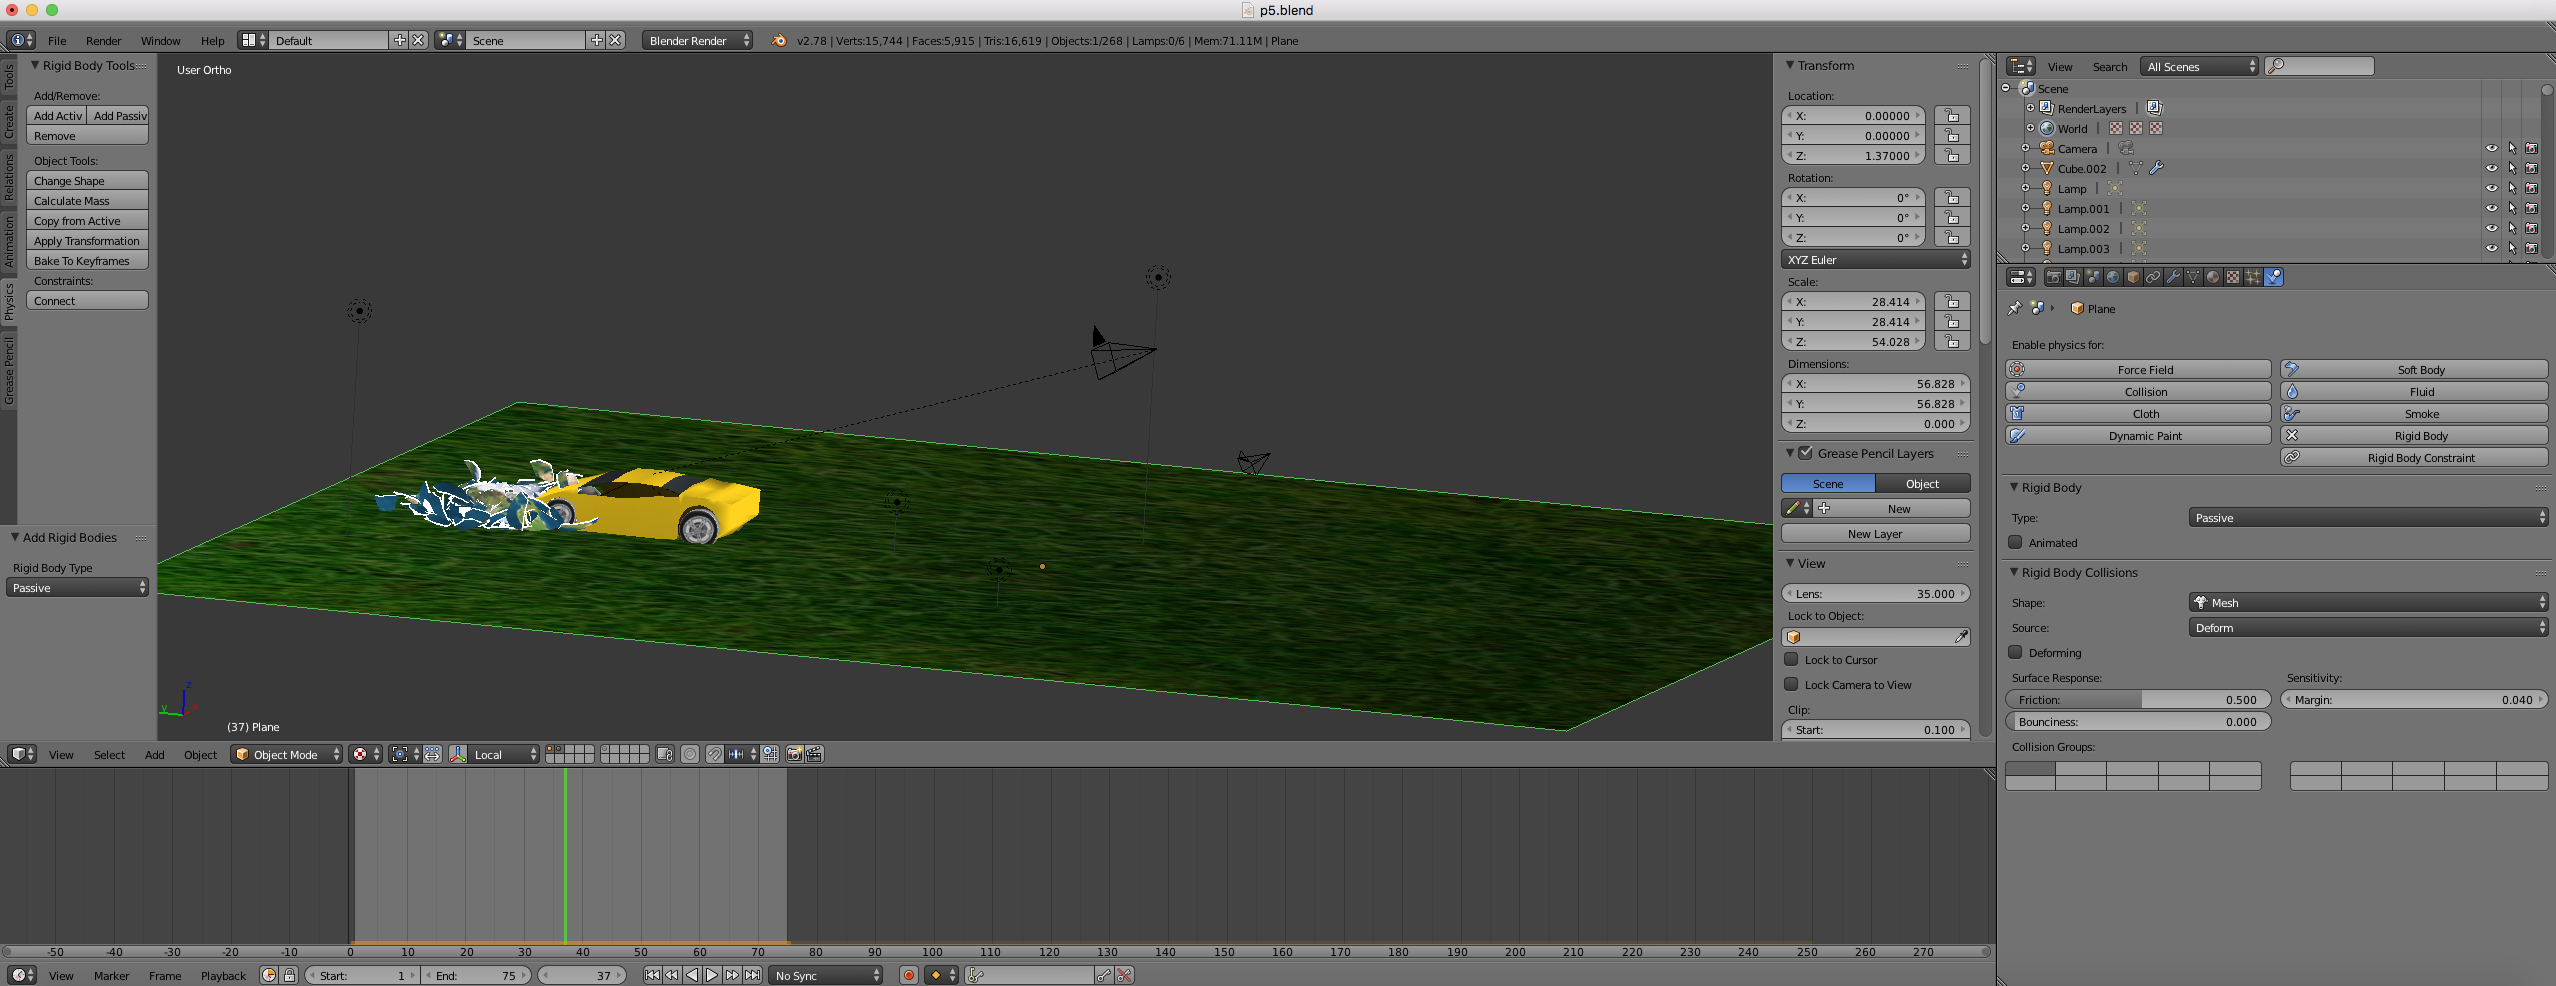
\includegraphics[width = 1.00\textwidth]{Imagenes/p5-img22}
 		\captionof{figure}{\label{fig:IPN}Simulando colisión (V).}
	\end{center} 
\end{figure}

\begin{figure}[H]
	\begin{center}
	 		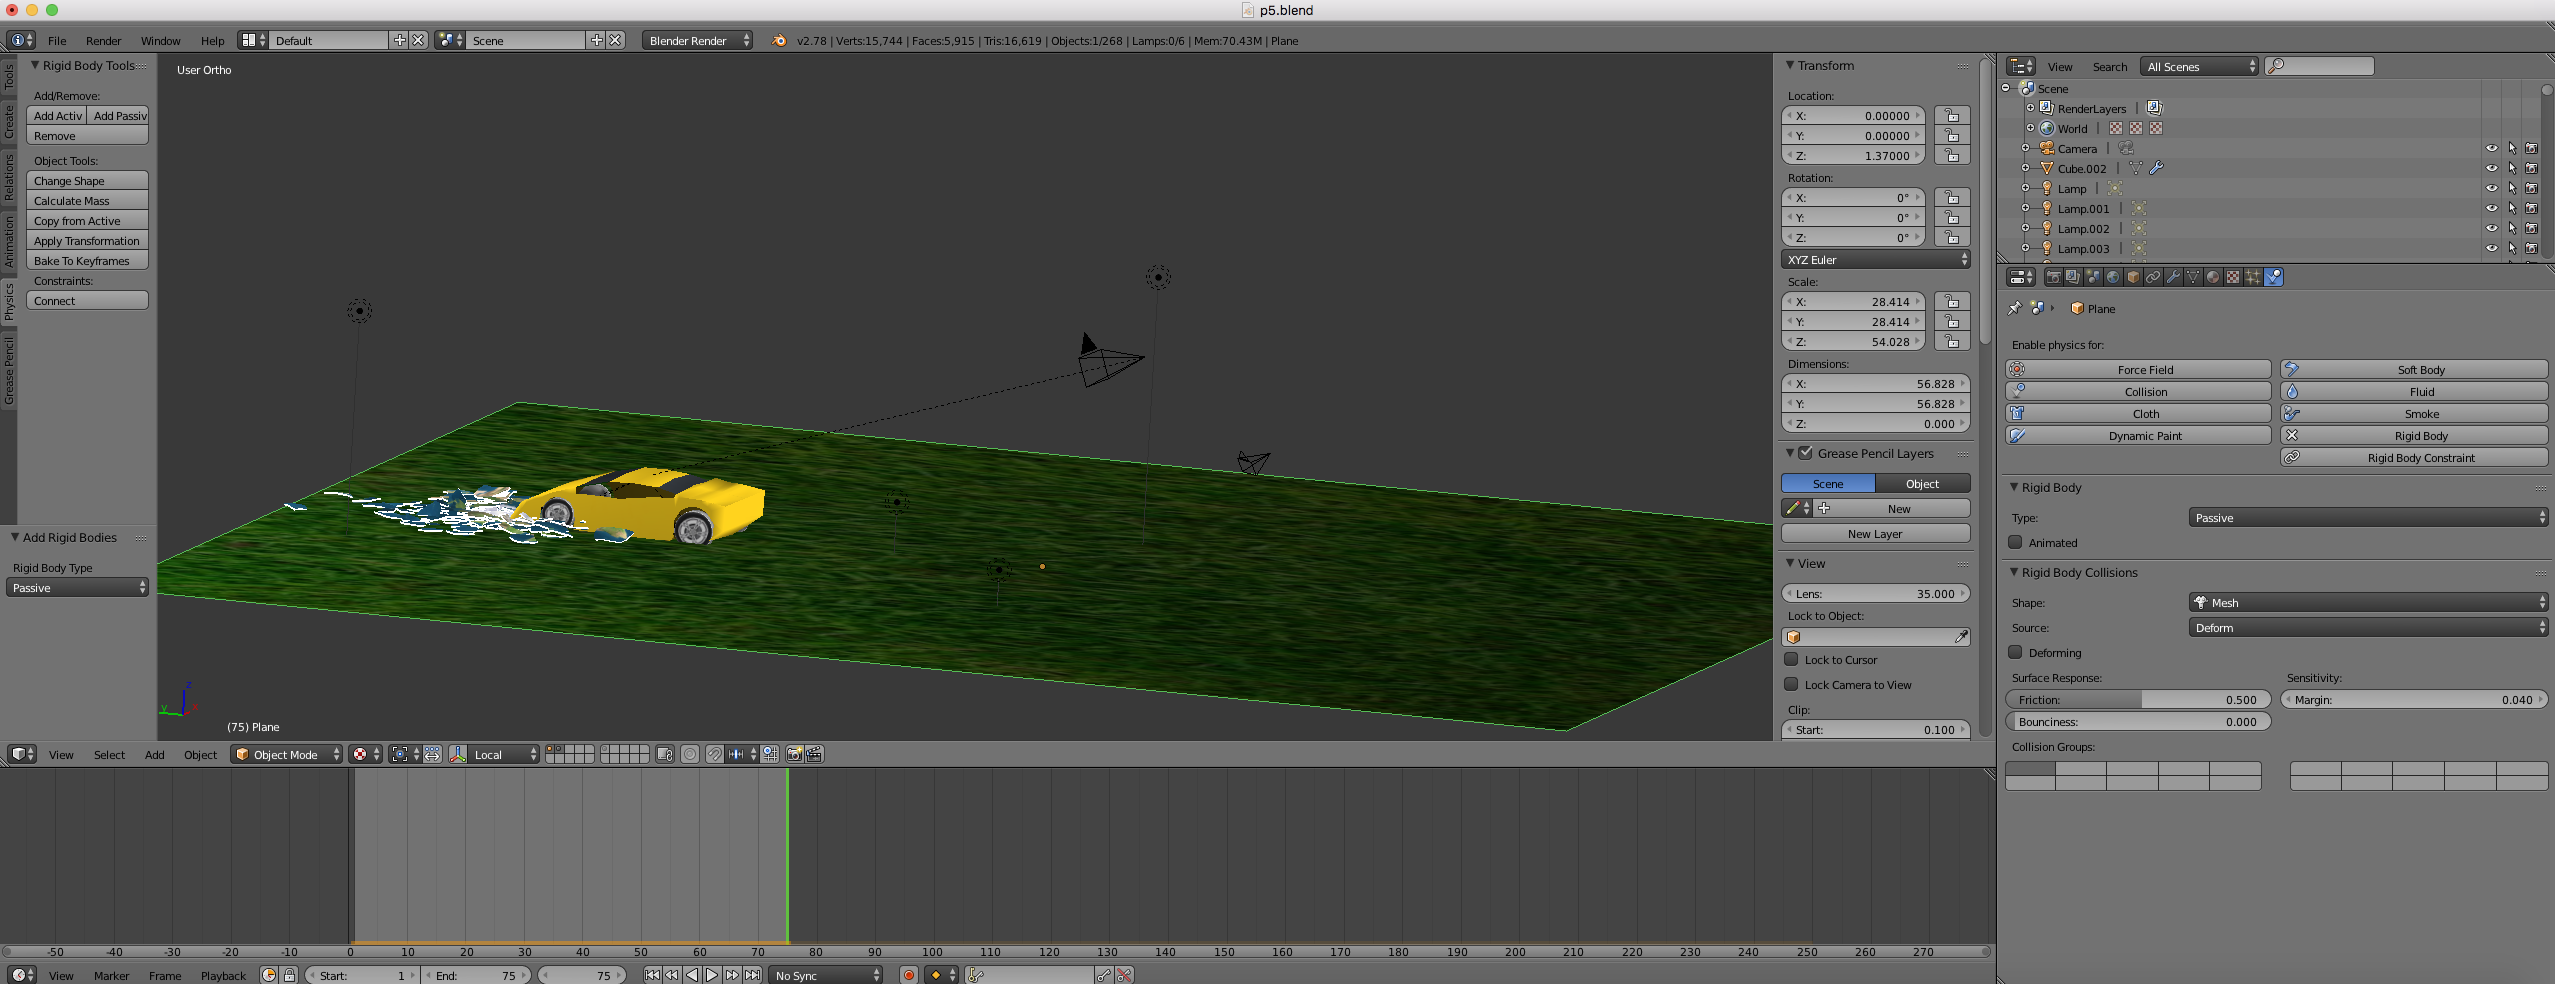
\includegraphics[width = 1.00\textwidth]{Imagenes/p5-img23}
 		\captionof{figure}{\label{fig:IPN}Simulando colisión (VI).}
	\end{center} 
\end{figure}

En el documento zip referente a la entrega de la práctica se encuentral fichero de blender correspondiente a la misma y la memoria donde se detallan los pasos realizados.

\end{document}